\clearpage

%\section {Neutrino oscillation fitting}
%\label{sec:oscfit}
%--------------------------------------------------------------------------------------------------------------------

\section {Sensitivity to $\bar{\nu}_e$ appearance}
\label{sec:sensitivity}

As discussed within the OA group, 
since there are not fitted parameters in the analysis, the validation can 
be done by comparing the rate-only with rate+shape p-values and 
checking if the corresponding distributions are reasonable.
Of course the final validation is given if all the oscillation analyses agree.
This is done by performing a sensitivity study to $\bar{\nu}_e$ appearance
both with the Asimov dataset, which consists of the most probable dataset
that is the nominal expected reconstructed energy distribution ~\cite{Asimov},
as well as for toy distributions, given a value of $\beta$.

The significance to $\bar{\nu}_e$ appearance is quoted for 
\TotalPot POT
%both \FakePotLow and 
%\FakePotHigh POT
using the procedure described in sec.~\ref{sec:pvalue}.
In order to quote the significance to $\bar{\nu}_e$ appearance a 1-sided p-value (right tail) is computed.
In addition a mean p-value is also computed by performing \NumToysLarge.

%--------------------------------------------------------------------------------------------------------------------

\subsection {Asimov rate-only p-value}
\label{subsec:rateonly}

The expected Asimov rate-only p-value is given by the Asimov dataset for $\beta=1$. 
The corresponding oscillation parameters are shown in table~\ref{tab:osc_params_fixed_values_reactor},
The distribution of the number of superK events used as test statistic is shown in figure~\ref{fig:pvalue_rateonly}. 
The number of events is
%3.718 for \FakePotLow POT 
%and 4.183 for  \FakePotHigh POT. 
%The quoted p-value is 
%and 0.113 for \FakePotLow POT.
%and 0.0538 for \FakePotHigh POT.
3.729 for \TotalPot POT
and the quoted p-value is 0.109.
In table~\ref{tab:summary_sensi_rateonly_highpot} the rate-only p-value is shown
for different numbers of observed events.

\begin{figure}
\center
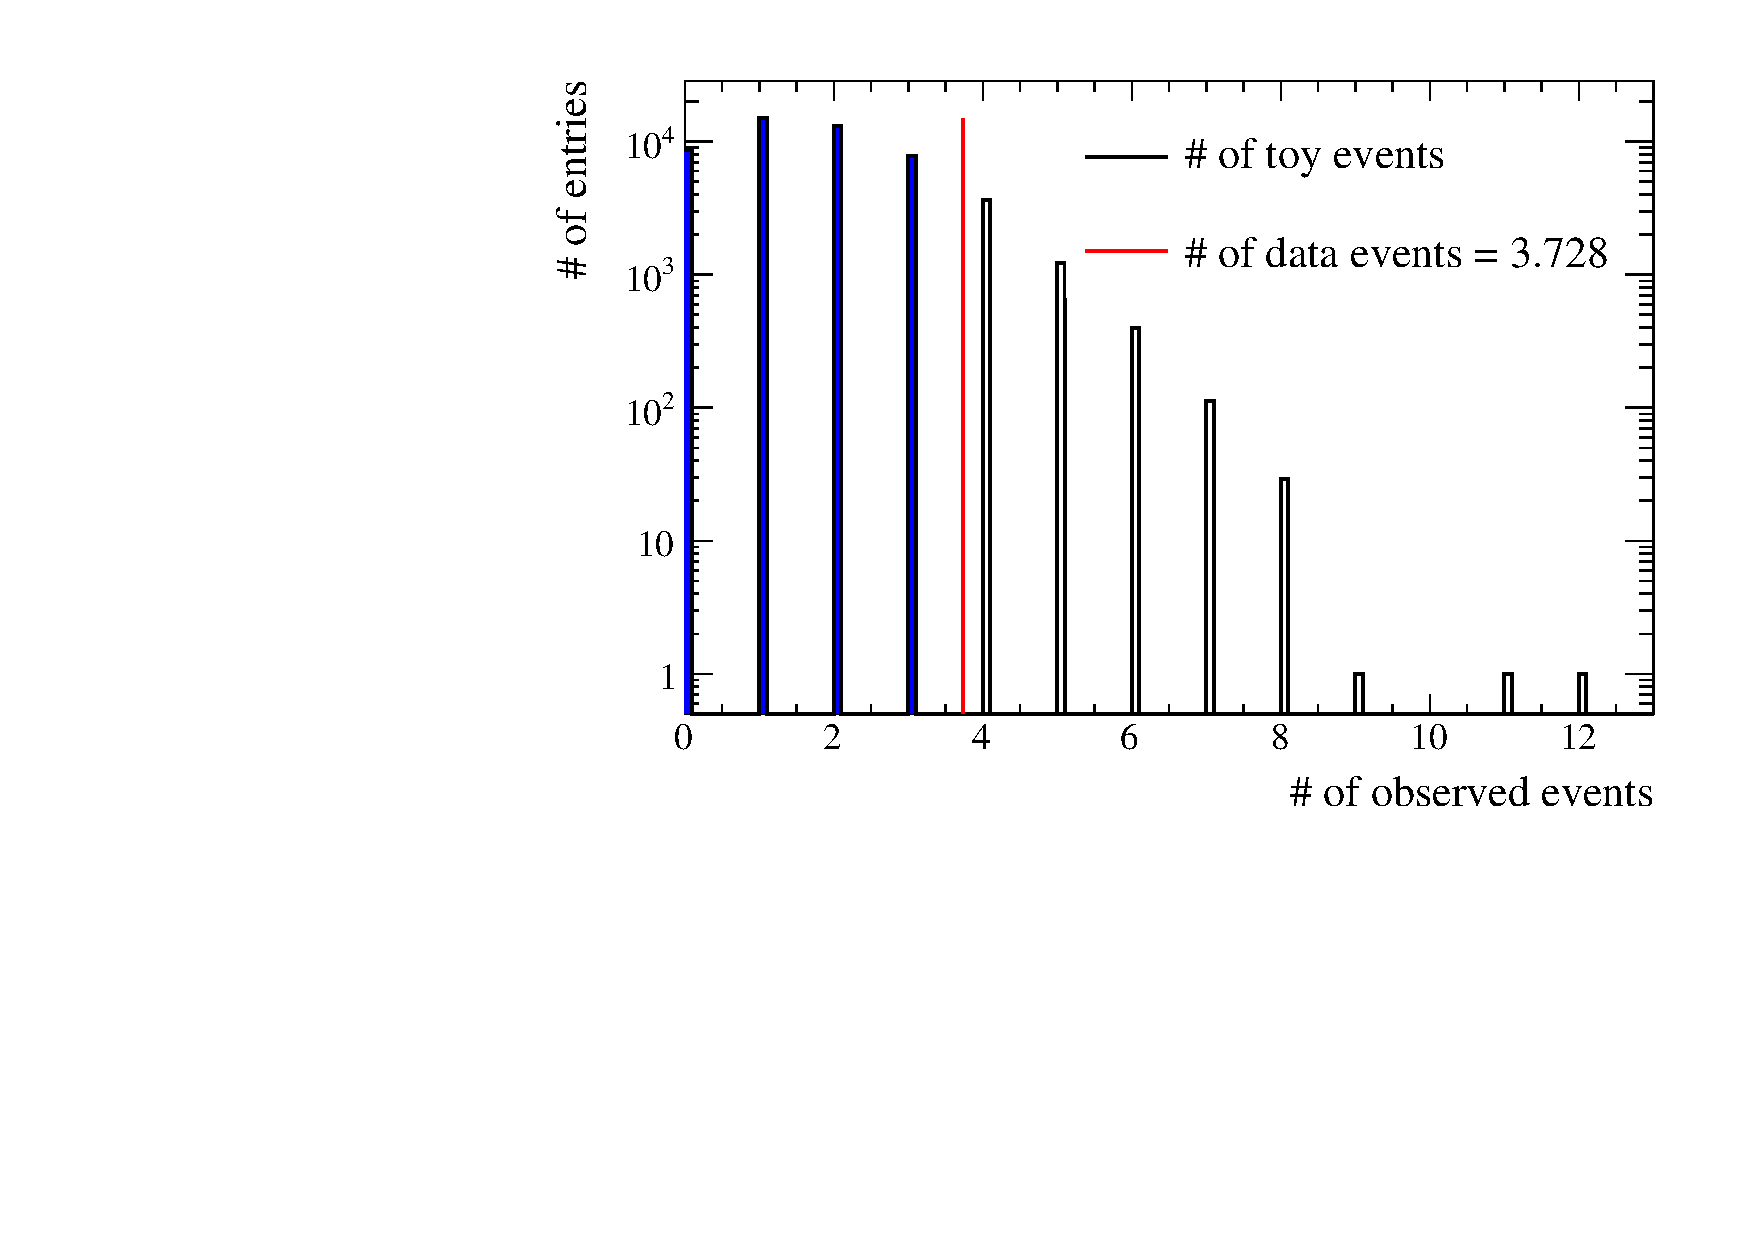
\includegraphics[width=0.48\linewidth]{./nuebar_plots/pvalue_median/pvalue_rate_4p0108E20POT_50ktoys.pdf}
%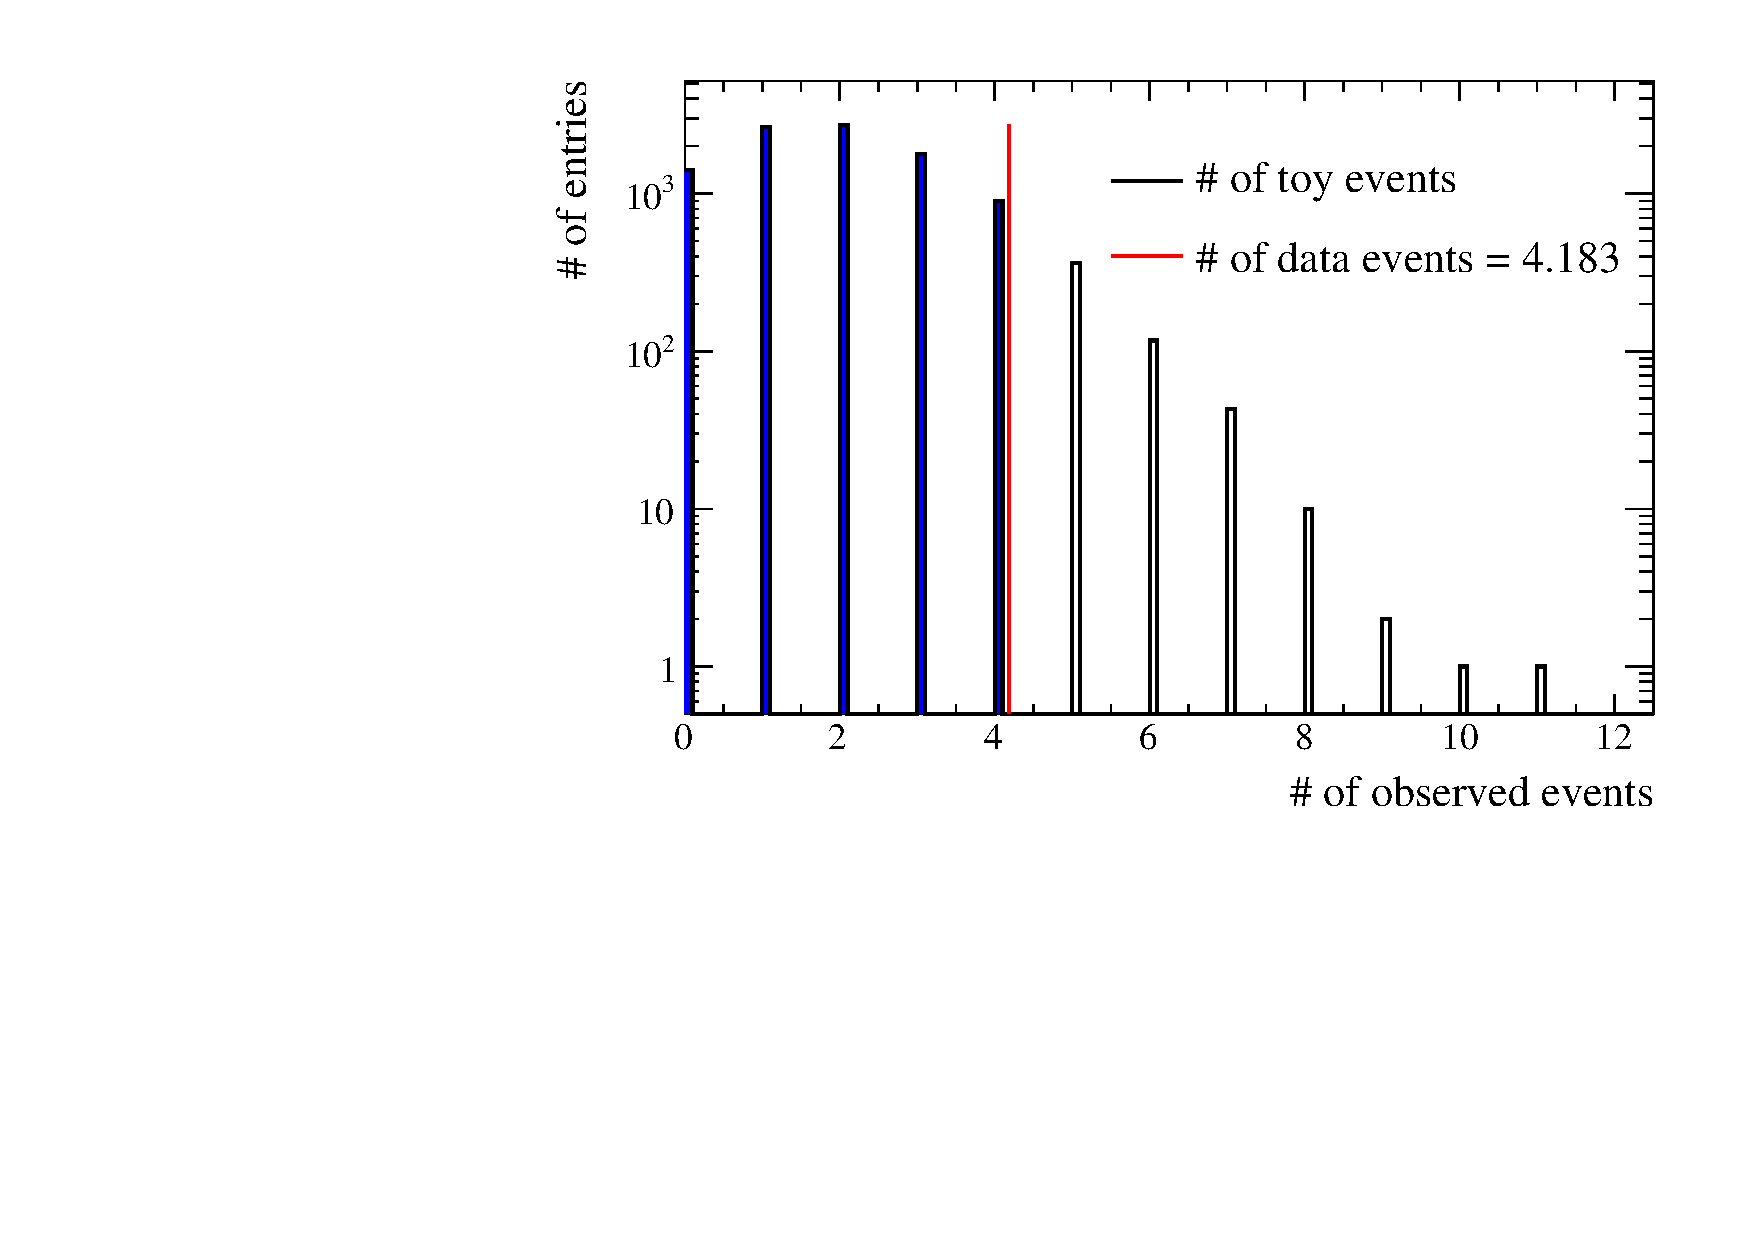
\includegraphics[width=0.48\linewidth]{./nuebar_plots/pvalue_median/pvalue_rate_4p5E20POT.pdf}
\caption {
The distribution of the total number of events from each of the \NumToysLarge toy experiments. 
The red line corresponds to the total number of events given by the Asimov dataset. 
The study is done with \TotalPot POT.
%\FakePotLow POT (left) and \FakePotHigh (right).
}
\label{fig:pvalue_rateonly}
\end{figure}

%--------------------------------------------------------------------------------------------------------------------




\subsection {Asimov rate+shape p-value}
\label{subsec:rateshape_median}

The $\chi^2$ distributions for both $\beta=0$ and $\beta=1$ are shown in figure~\ref{fig:chisq_rateshape}.
%
\begin{figure}
\center
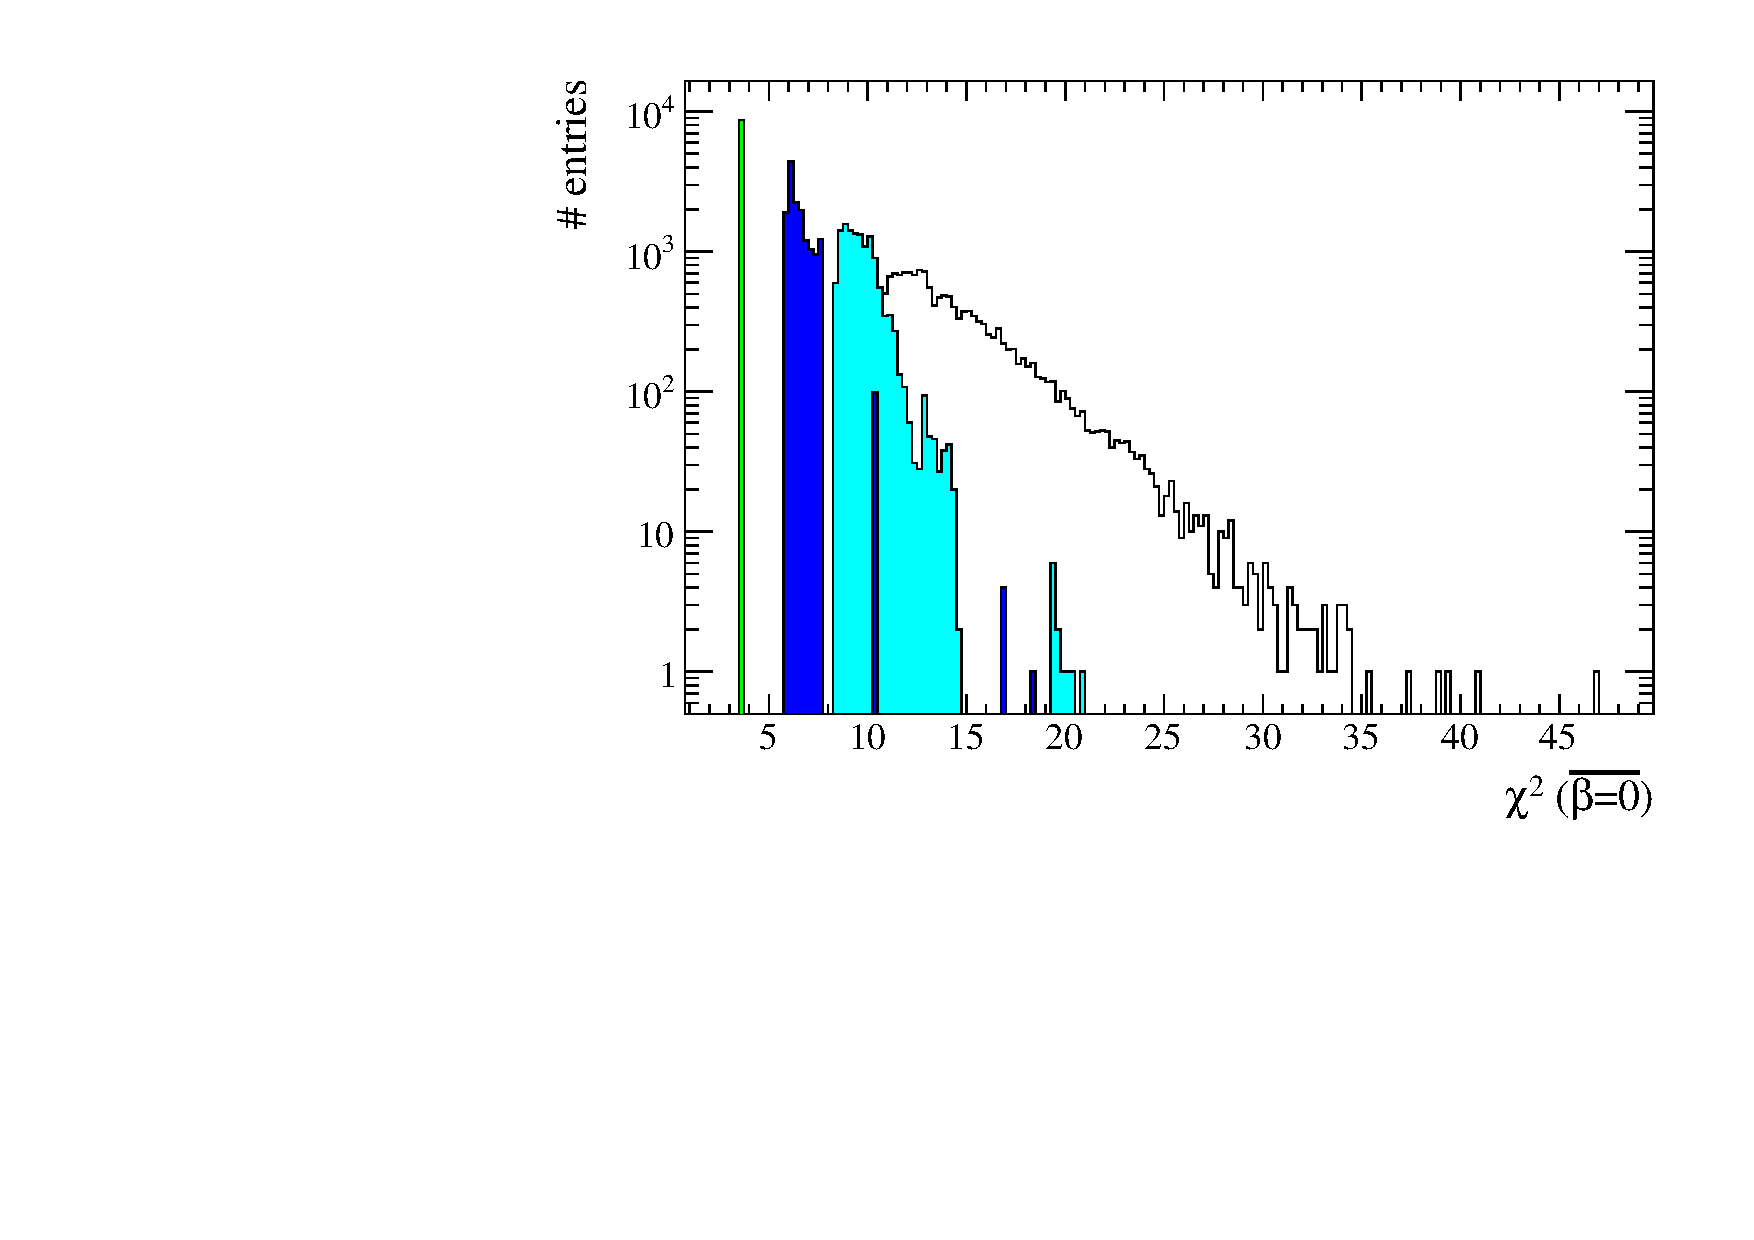
\includegraphics[width=0.48\linewidth]{./nuebar_plots/pvalue_median/chisq_beta0_4p0108E20POT_50ktoys.pdf}
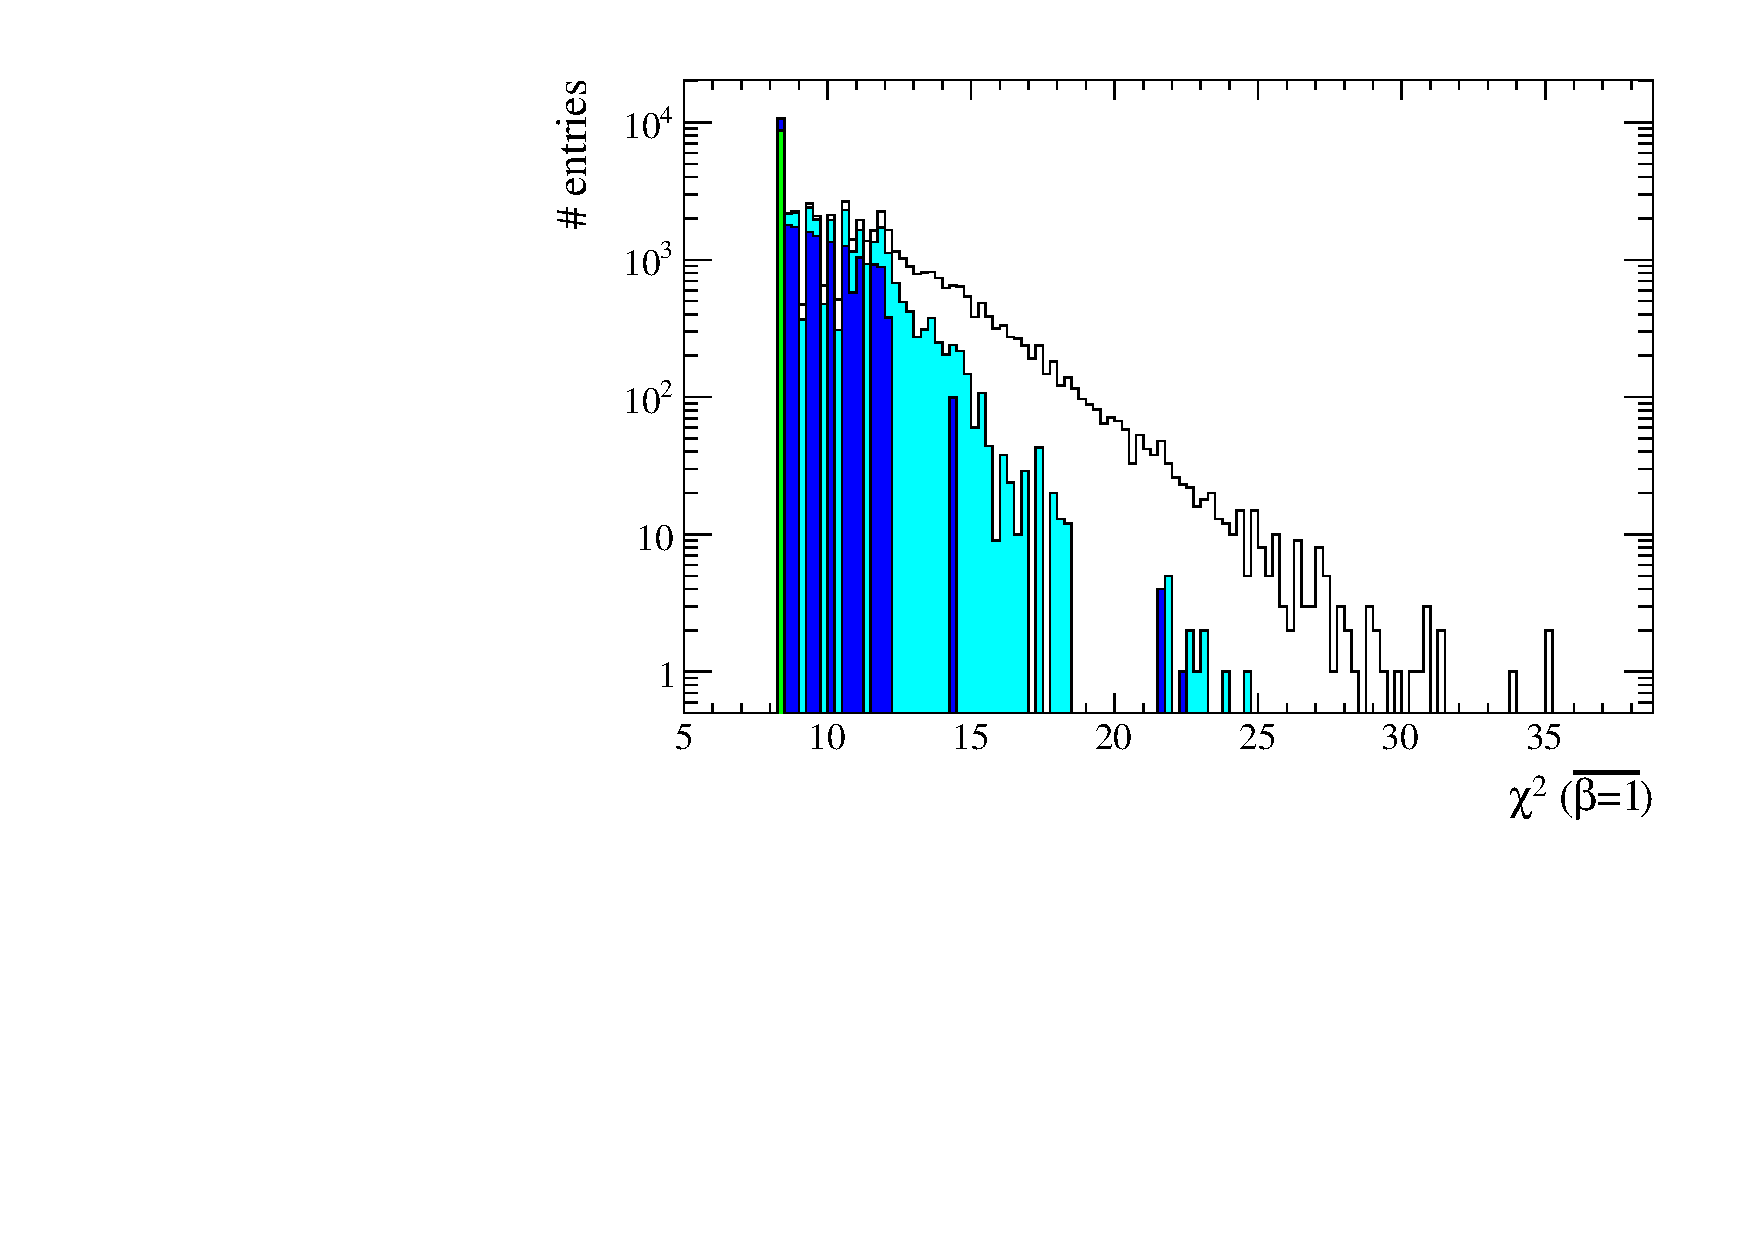
\includegraphics[width=0.48\linewidth]{./nuebar_plots/pvalue_median/chisq_beta1_4p0108E20POT_50ktoys.pdf}
\caption {
Distribution of the $\chi^2$ for $\beta=0$ (left) and $\beta=1$ (right).
They correspond to \TotalPot POT.
%\FakePotHigh POT.
The colored green entries correspond to the toys with no observed events while the 
blu and the cyan entries correspond respectively to toys with 1 and 2 events.
\NumToysLarge toys are used.
}
\label{fig:chisq_rateshape}
\end{figure}
%
They don't follow a real $\chi^2$ distribution because the number of events is low,
as explained in sec.~\ref{sec:oscfit_method}.
In particular it is visible that the region where spikes are present is dominated 
by a low number of events, between 0 and 2. 
Since the statistical uncertainty is very large and dominant, 
the shape information cannot be fully exploited
and the distributions partially show a discrete behavior. 
Indeed if the statistics is increased to the expected full T2K number of POT, \TargetFullPot,
the distributions behave as a $\chi^2$ function with 25 degrees of freedom 
(the number of reconstructed energy bins), as expected.
This is shown in figure~\ref{fig:chisq_rateshape_fullpot}.

\begin{figure}
\center
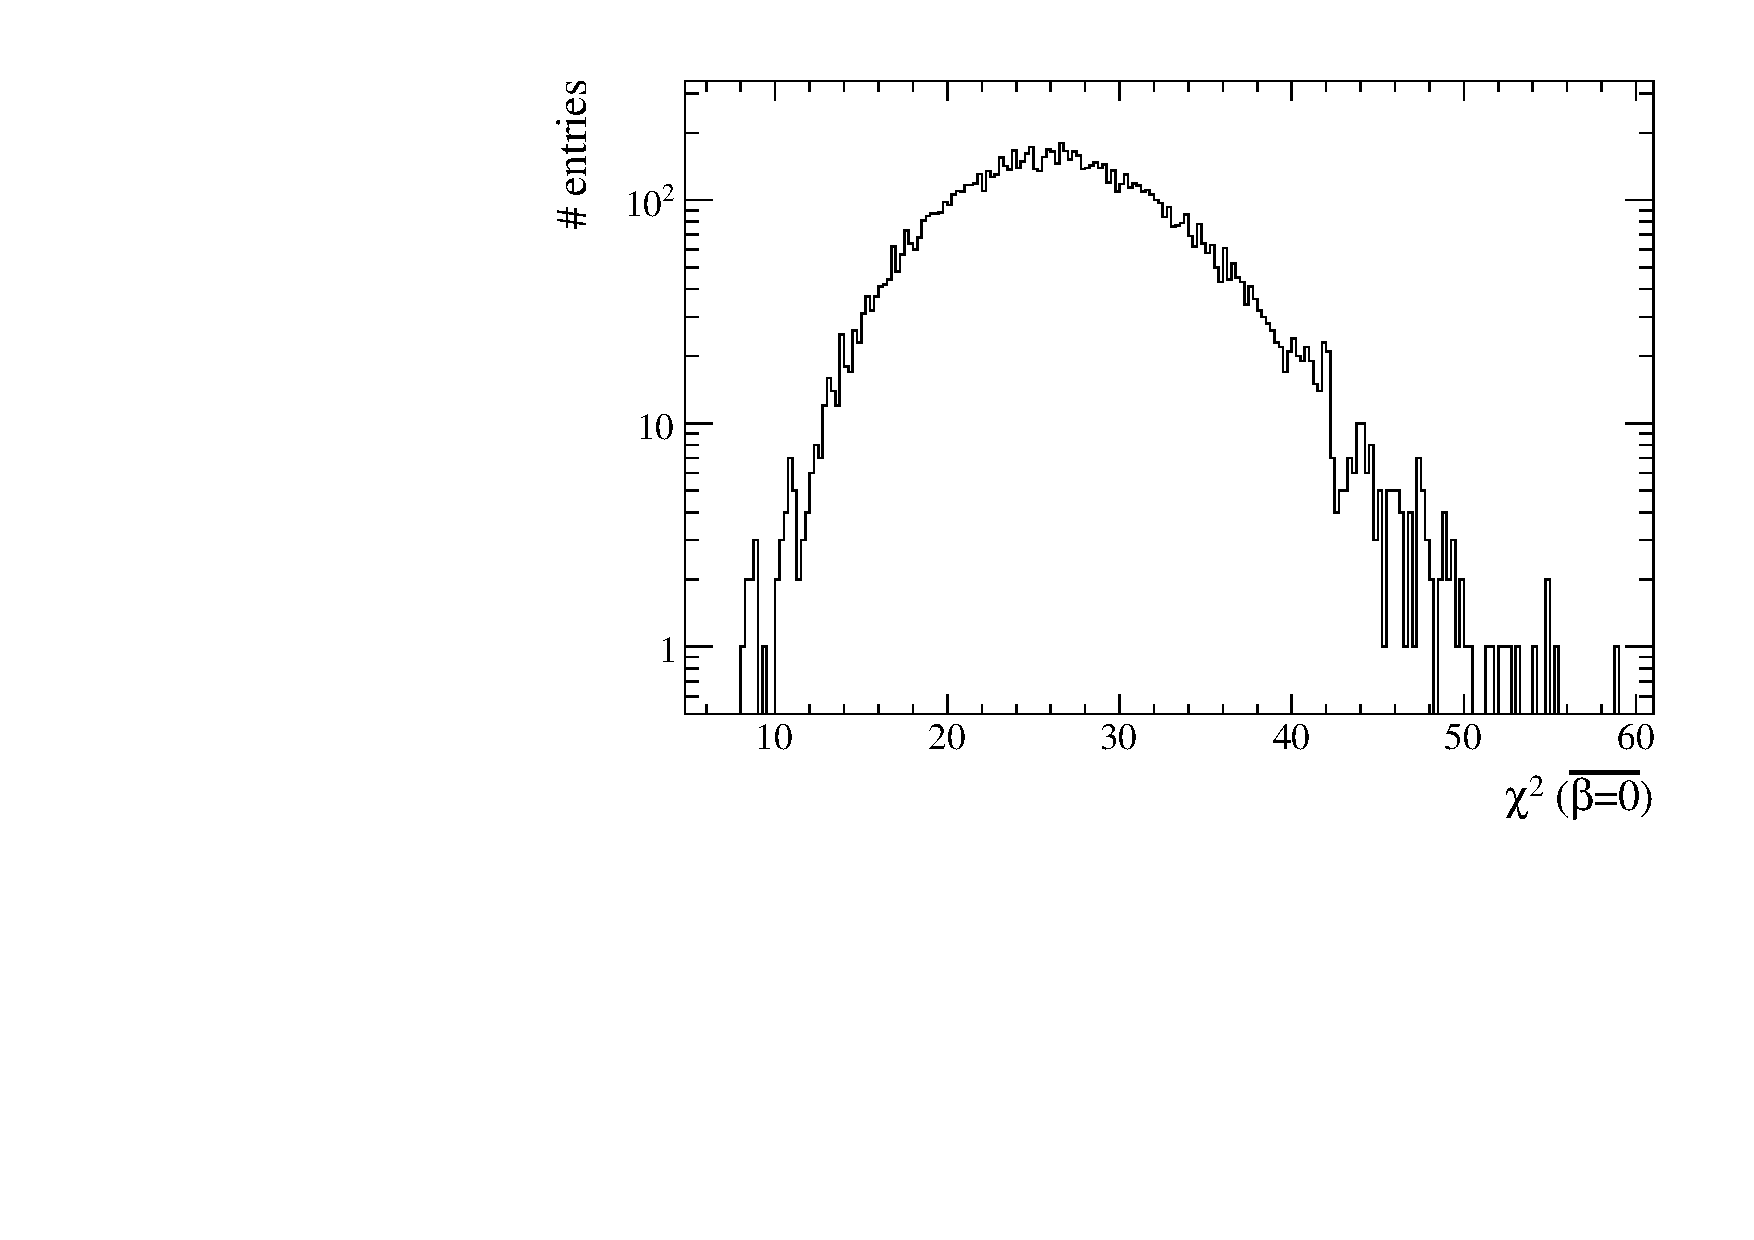
\includegraphics[width=0.48\linewidth]{./nuebar_plots/sensitivity/chisq_0_rateshape_T2Kfull.pdf}
%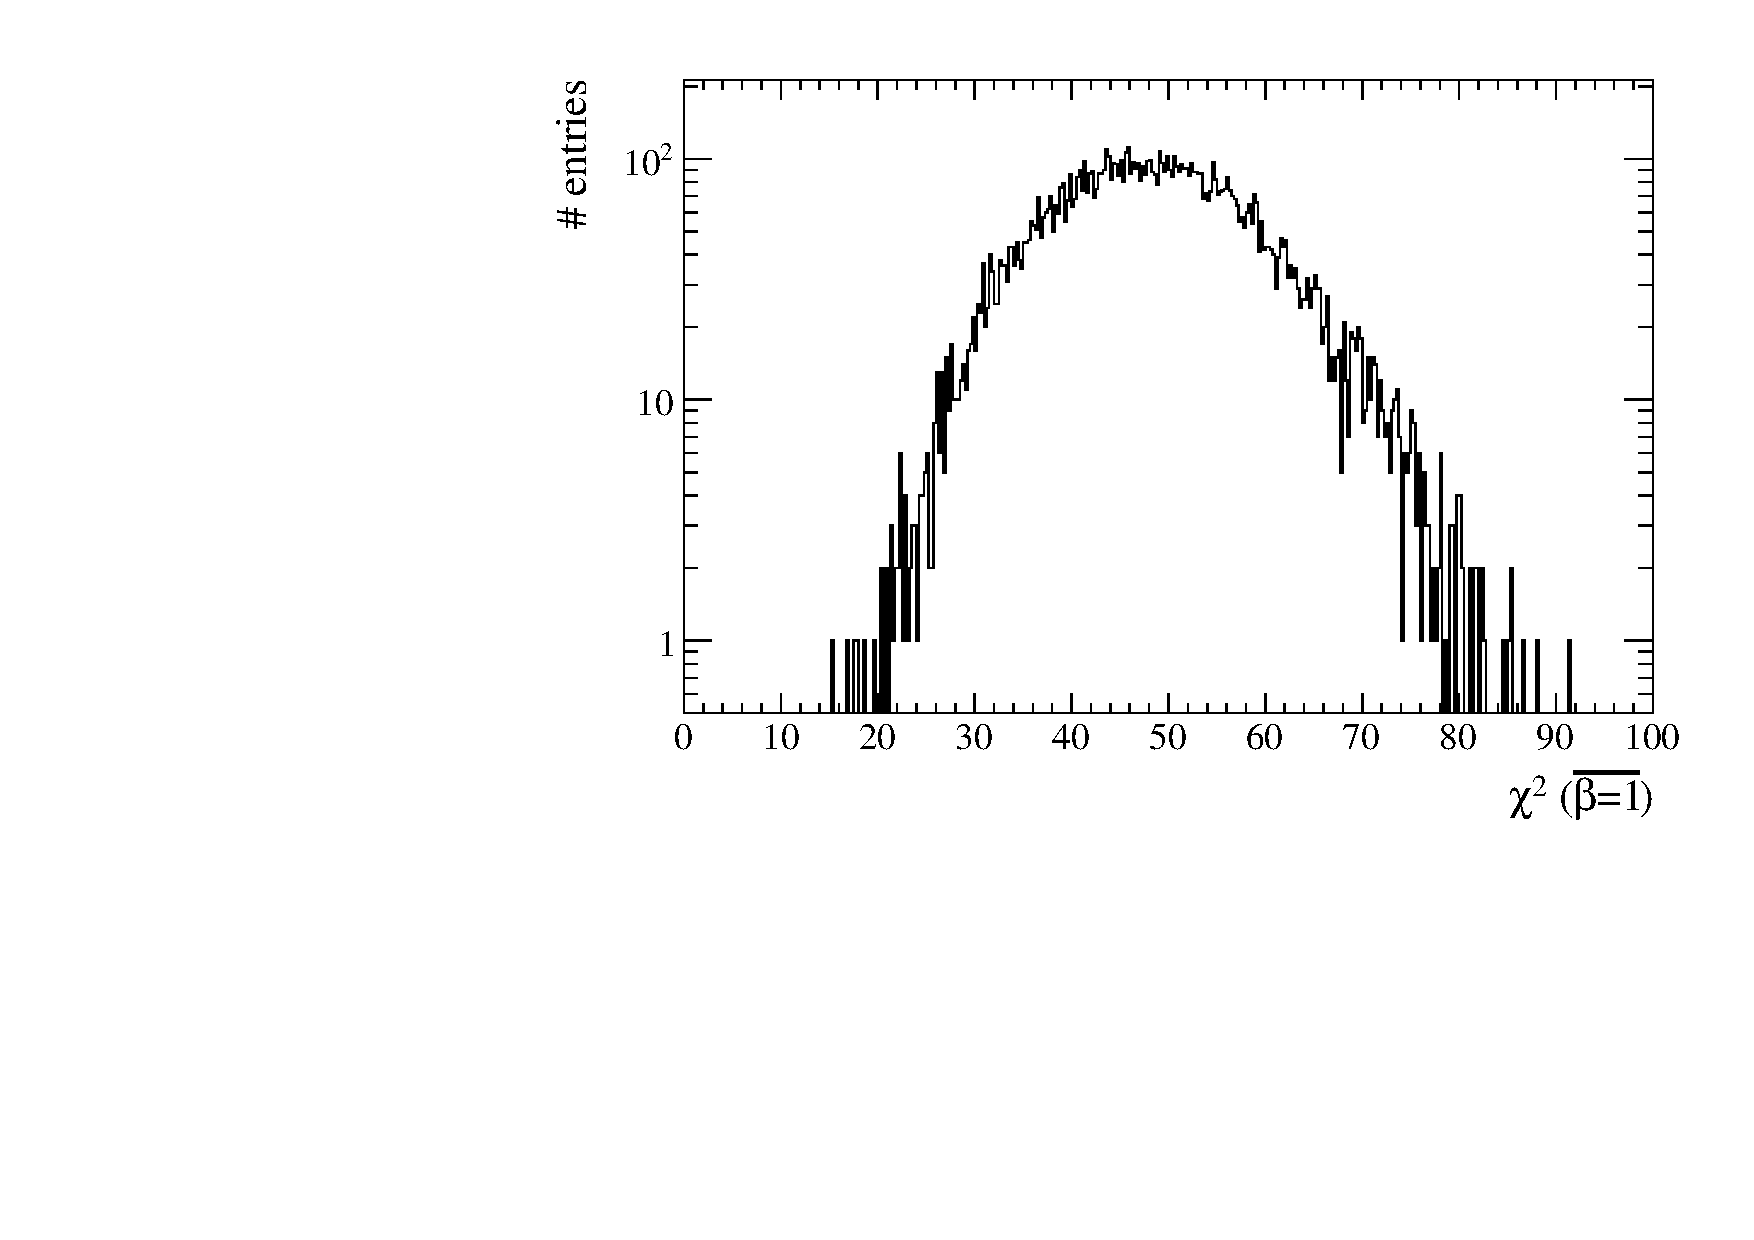
\includegraphics[width=0.48\linewidth]{./nuebar_images/sensitivity/chisq_1_rateshape_T2Kfull.pdf}
\caption {
Distribution of the $\chi^2$ for $\beta=0$. % (left) and $\beta=1$ (right).
They correspond to \TargetFullPot POT.
\NumToys toys are used.
%\newline
%{\bf TO UPDATE}
%\newline
}
\label{fig:chisq_rateshape_fullpot}
\end{figure}

The expected distribution of $\Delta \chi^2$ for all the \NumToysLarge toy experiments
is shown in Fig.~\ref{fig:pvalue_rateshape} for 
\TotalPot POT.
%both \FakePotLow and 
%\FakePotHigh POT.
%p-value given by the Asimov dataset for $\beta=1$ (PMNS expectation)
%The $\Delta \chi^2$ from the Asimov dataset is 1.932 with \FakePotHigh POT,
%while for \FakePotLow it is 1.72185.
The $\Delta \chi^2$ from the Asimov dataset is 1.728.
The Asimov expected p-value
is 0.0699 for \TotalPot POT.
%are 0.0723 for \FakePotLow POT
%and 0.0572 for \FakePotHigh POT.
%The rate-only p-value is smaller than the rate+shape p-value 
%because of the discrete behaviour of the test statistic in the rate-only analysis.
%This feature is discussed more in detail in Sec.~\ref{subsec:pvalue_mean}.
%\newline

\begin{figure}
\center
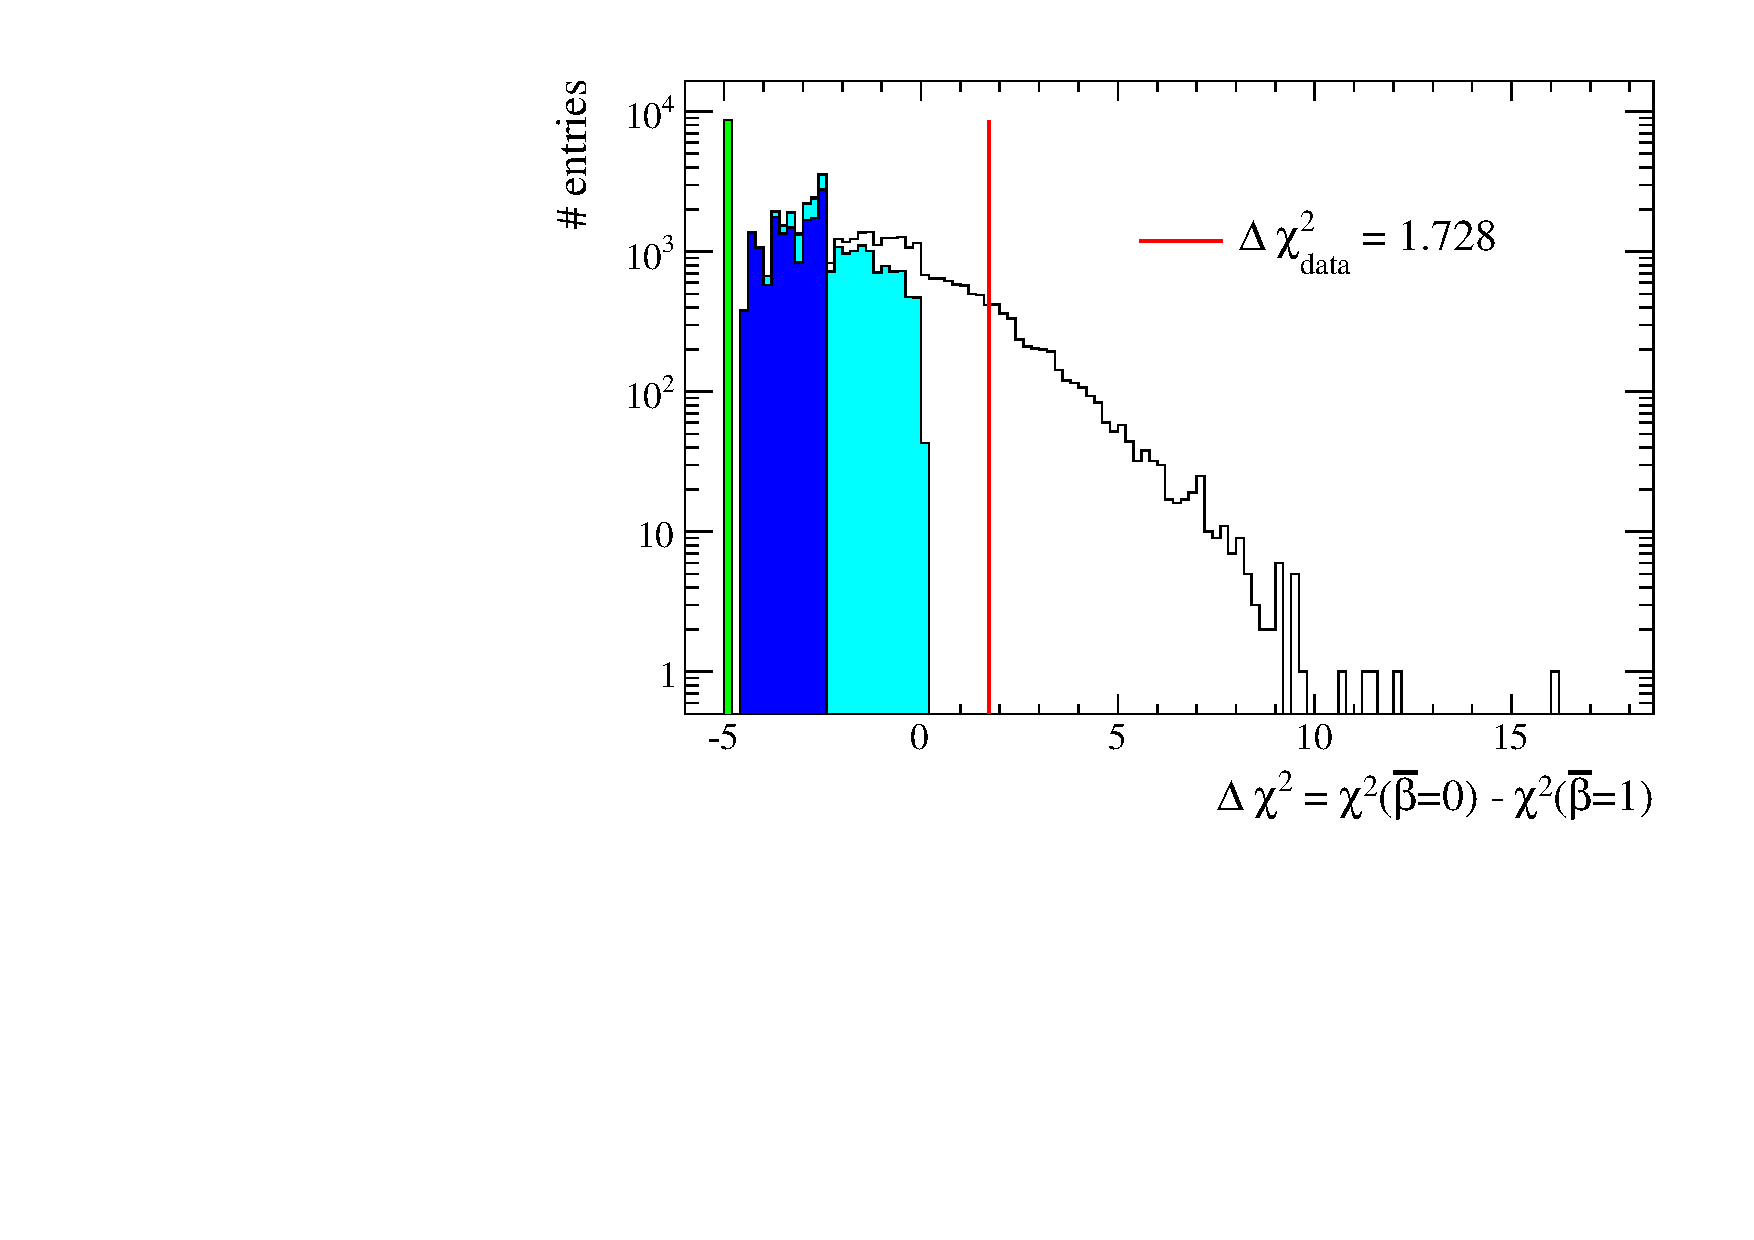
\includegraphics[width=0.48\linewidth]{./nuebar_plots/pvalue_median/deltachisq_4p0108E20POT_50ktoys.pdf}
%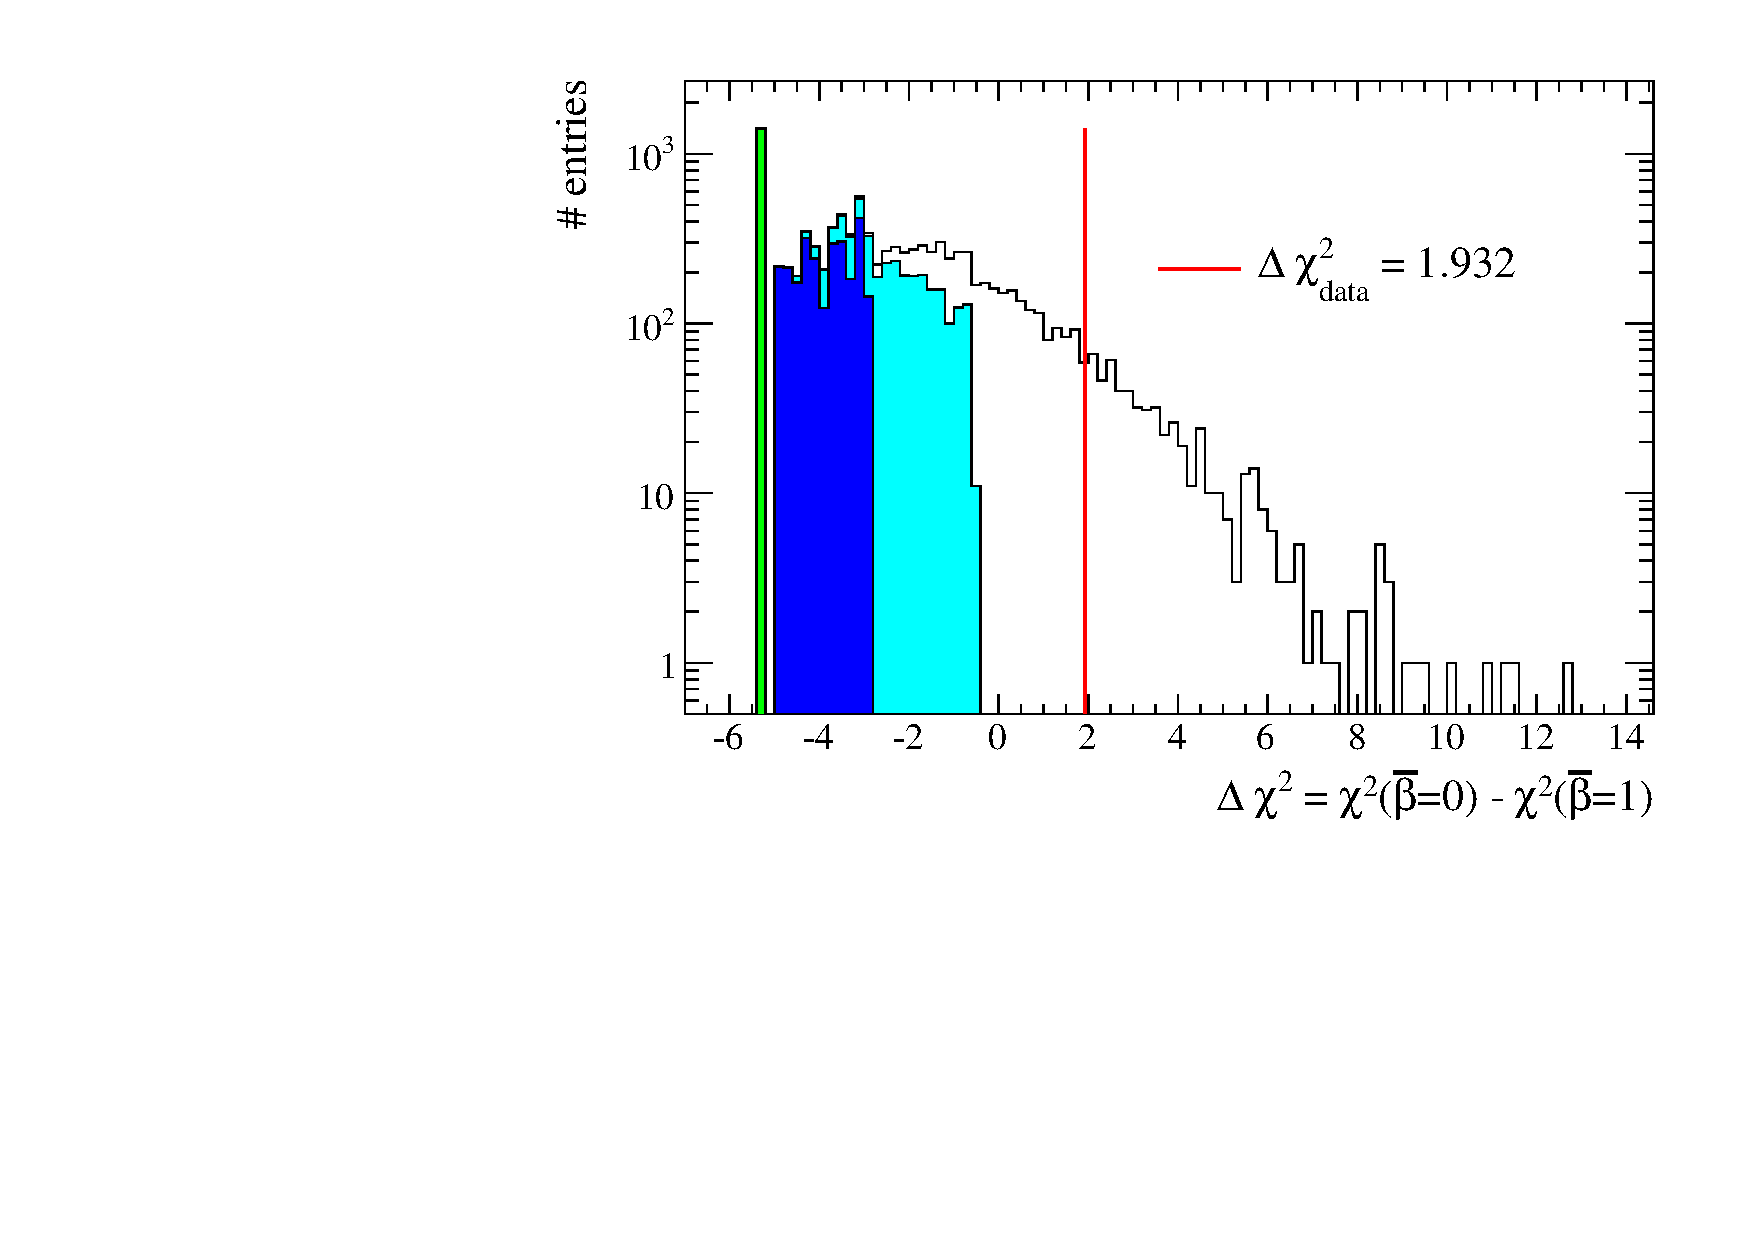
\includegraphics[width=0.48\linewidth]{./nuebar_plots/pvalue_median/deltachisq_4p5E20POT.pdf}
\caption {
Distribution of the $\Delta \chi^2$ for each of the \NumToysLarge toy experiment. 
The red line corresponds to $\Delta \chi^2$ obtained from the Asimov dataset. 
The study is done with 
\TotalPot POT.
%\FakePotLow POT (left) and 
%\FakePotHigh (right).
The colored green entries correspond to the toys with no observed events while the 
blu and the cyan entries correspond respectively to toys with 1 and 2 events.
}
\label{fig:pvalue_rateshape}
\end{figure}

The p-value for the Asimov dataset as a function of $\beta$ or the total number of events is shown for 
%\FakePotLow in fig.~\ref{fig:pvalue_Vs_beta_lowpot}, fig.~\ref{fig:pvalue_Vs_nevents_lowpot}
%\FakePotHigh respectively in fig.~\ref{fig:pvalue_Vs_beta_highpot} and fig.~\ref{fig:pvalue_Vs_nevents_highpot}.
\TotalPot POT in figure~\ref{fig:pvalue_Vs_beta_lowpot} and figure~\ref{fig:pvalue_Vs_nevents_lowpot}. 

\begin{figure}
\center
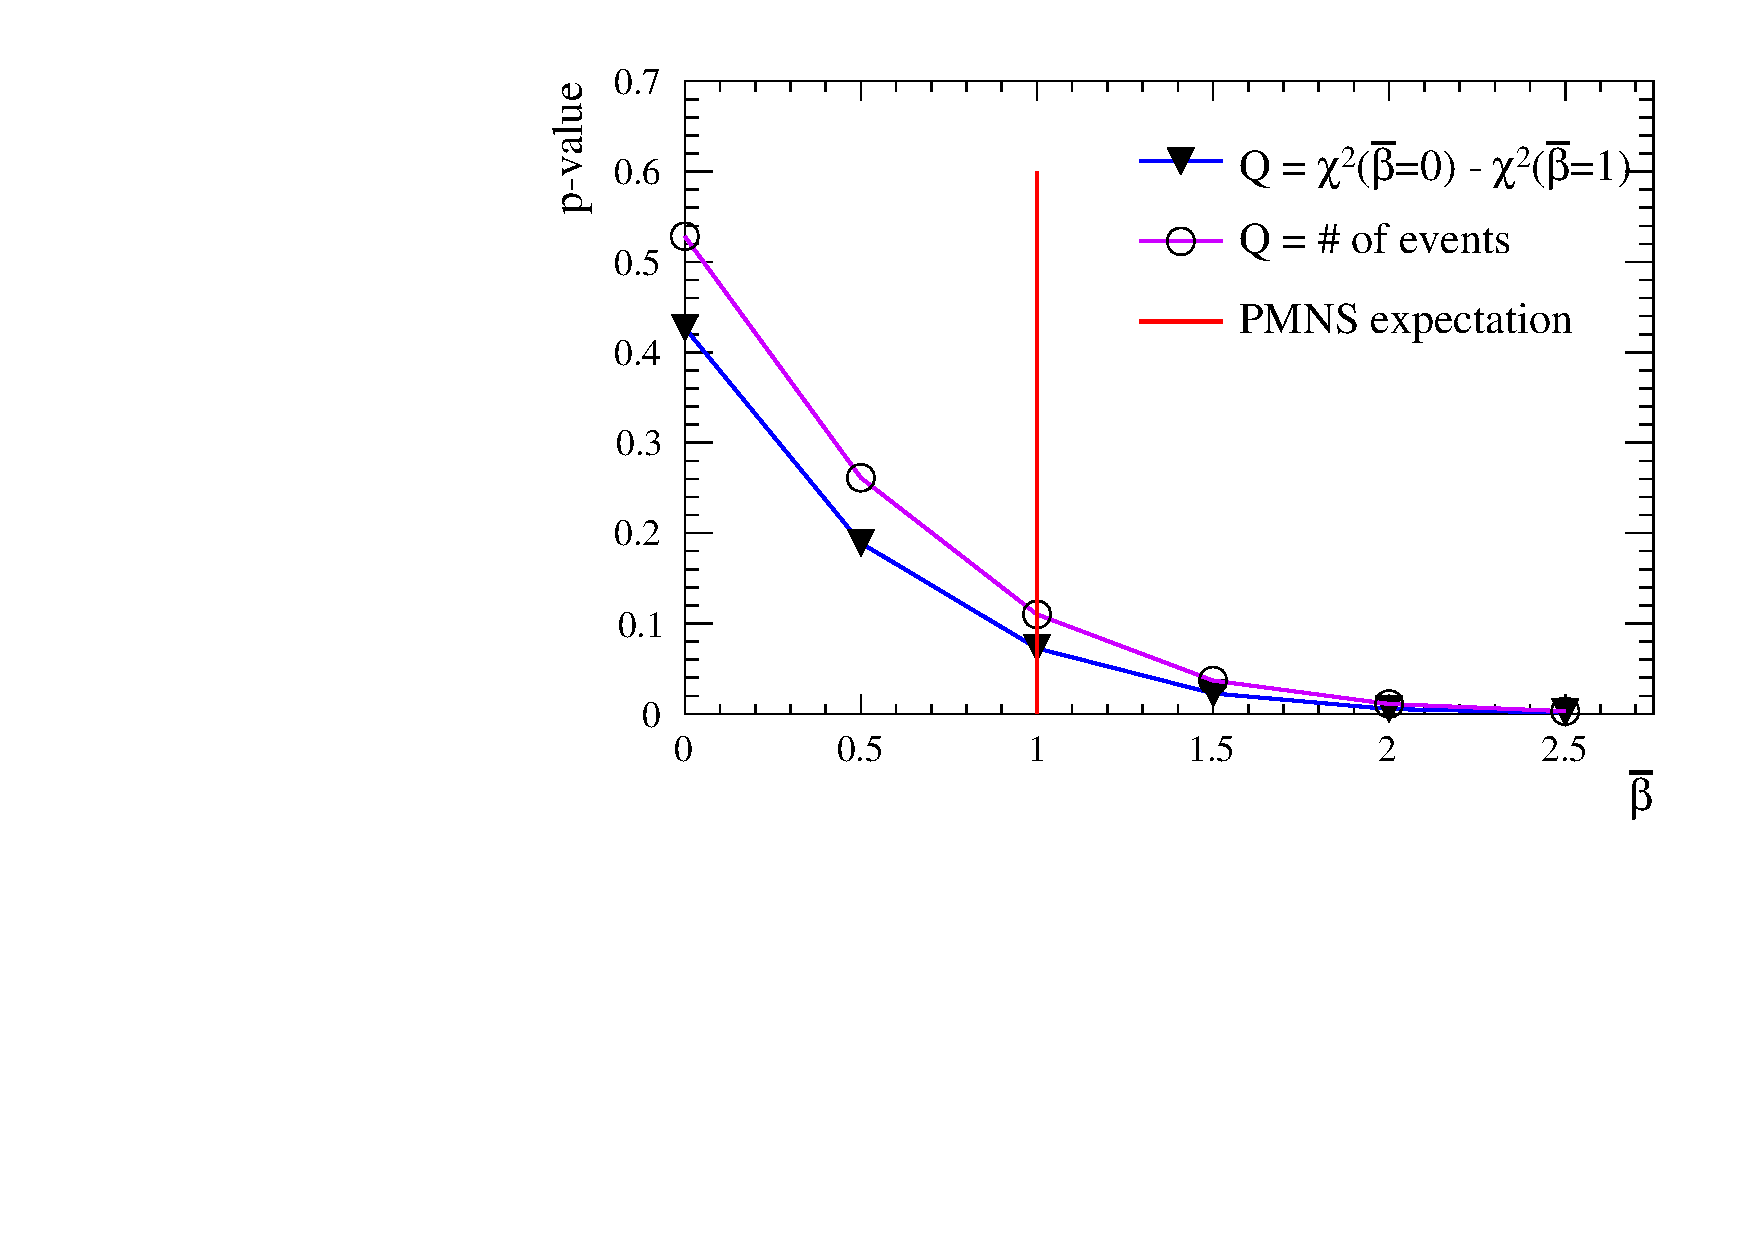
\includegraphics[width=0.48\linewidth]{./nuebar_plots/sensitivity/pvalue_Vs_beta_4p0108E20POT.pdf}
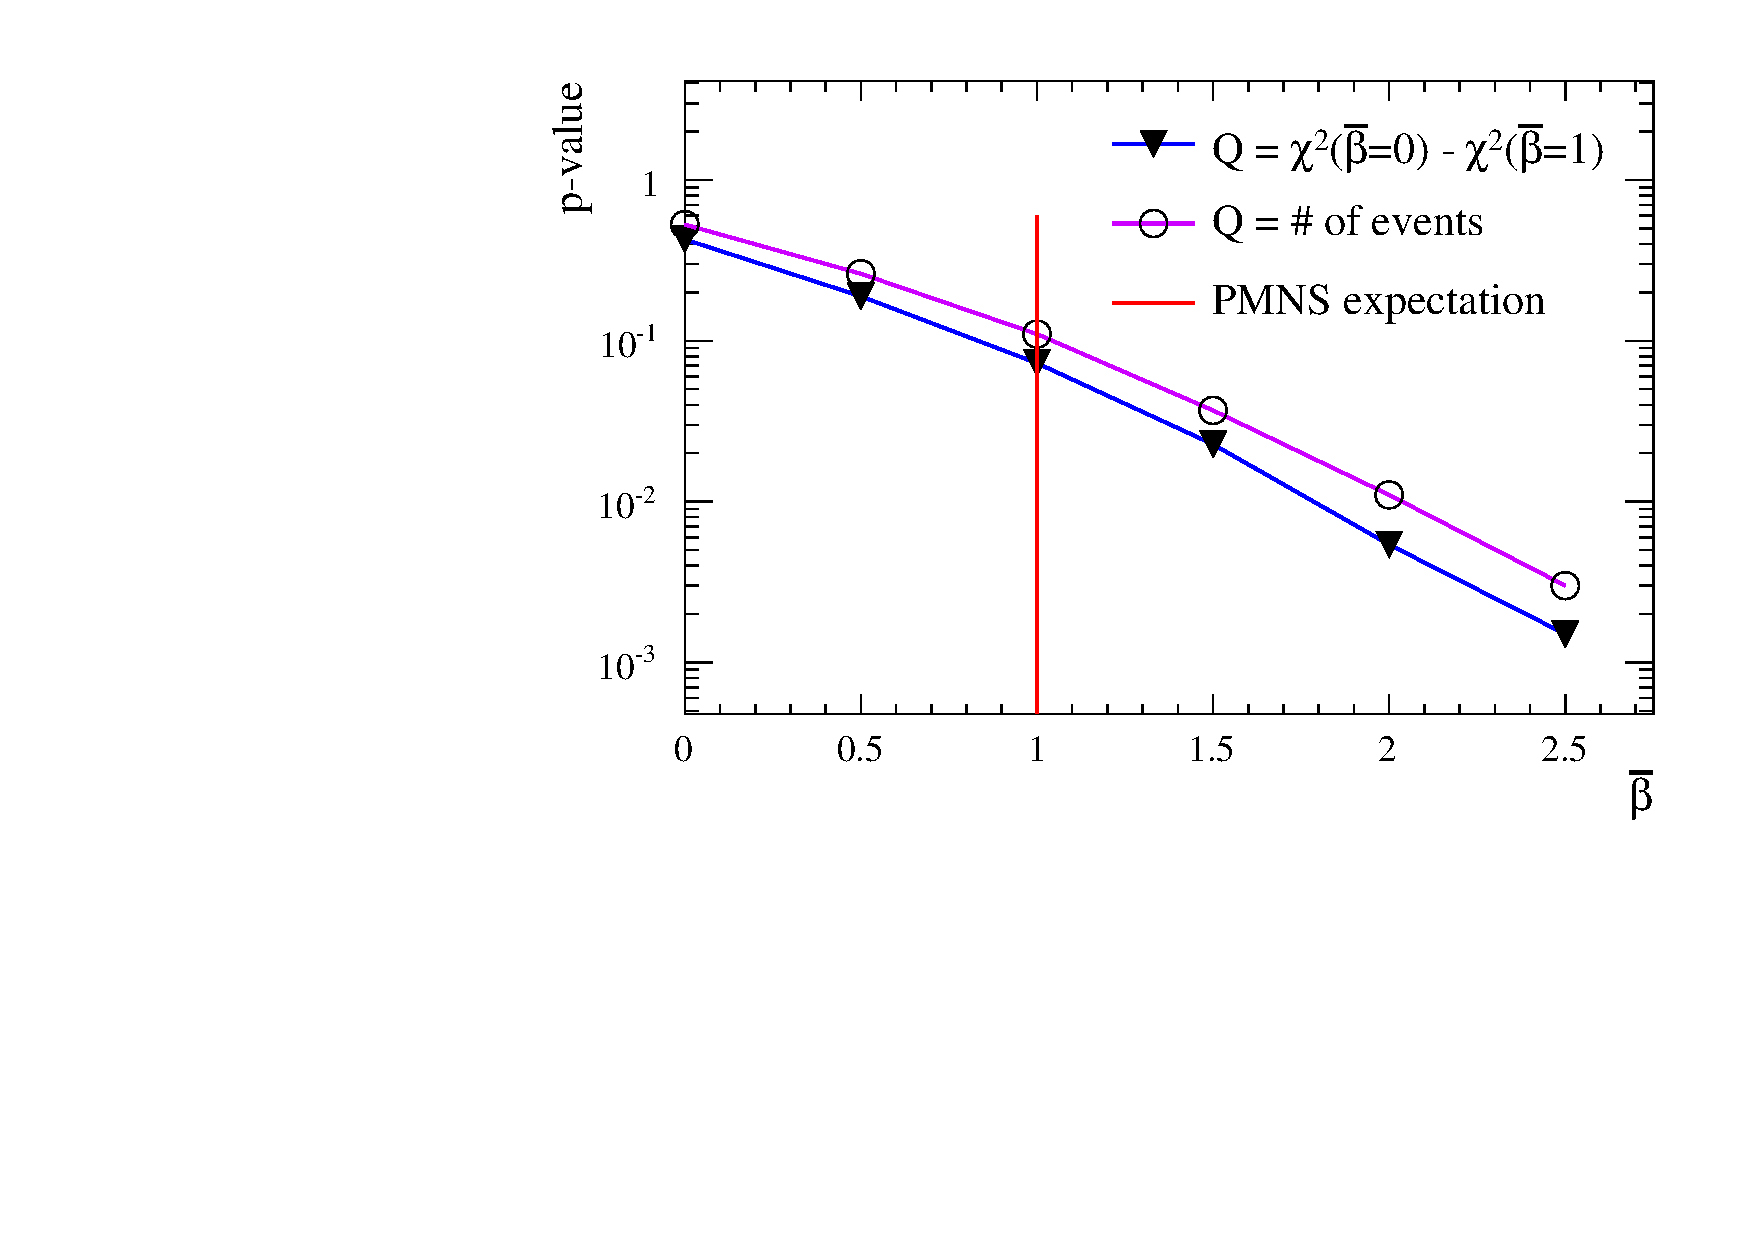
\includegraphics[width=0.48\linewidth]{./nuebar_plots/sensitivity/pvalue_Vs_beta_4p0108E20POT_log.pdf}
\caption {
Rate-only (violet) and rate+shape (blue) p-value given by Asimov datasets for several values of $\beta$
in normal (left) and logarithmic (right) scale.
The red line corresponds to the PMNS expectation ($\beta =1$).
%The study is done with \FakePotLow POT.
The study is done with \TotalPot POT.
\NumToys toys are used.
}
\label{fig:pvalue_Vs_beta_lowpot}
\end{figure}

\begin{figure}
\center
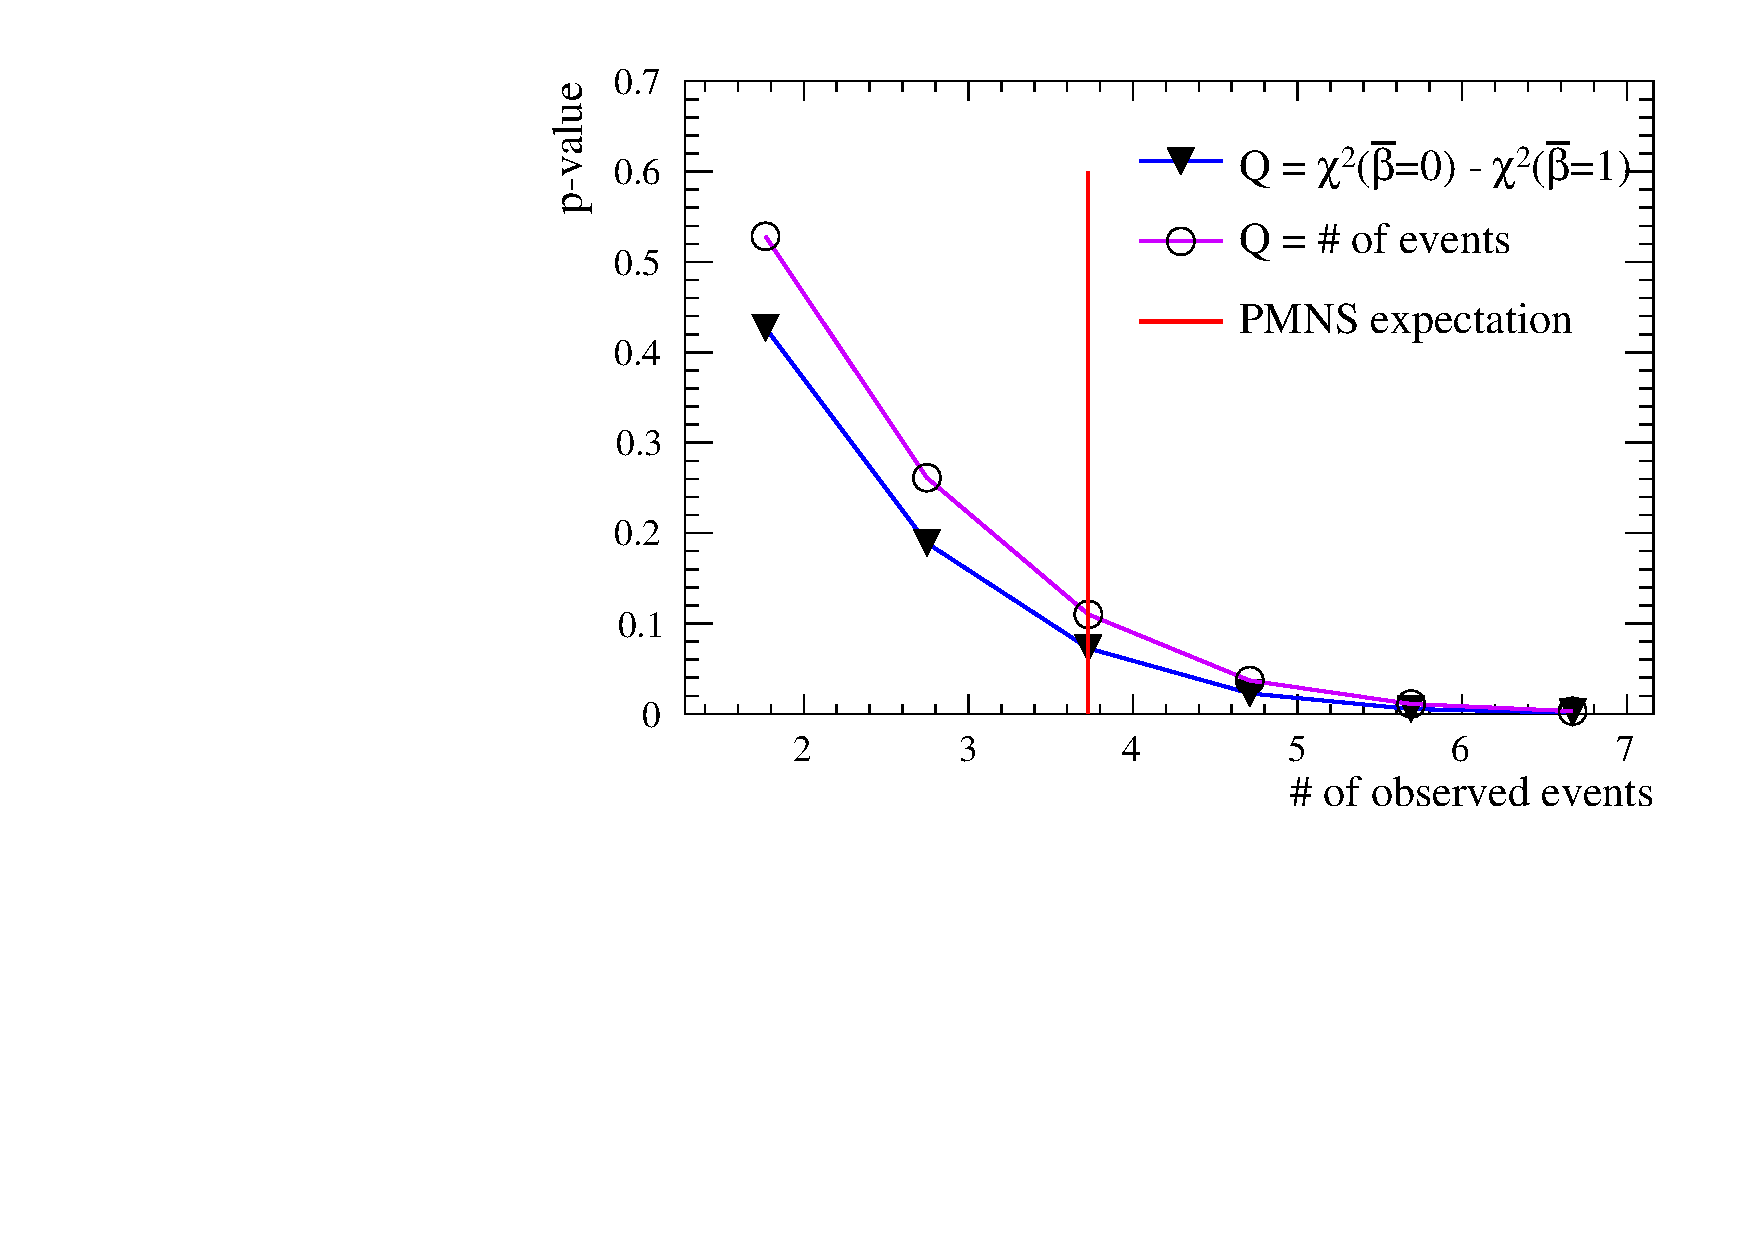
\includegraphics[width=0.48\linewidth]{./nuebar_plots/sensitivity/pvalue_Vs_nevents_4p0108E20POT.pdf}
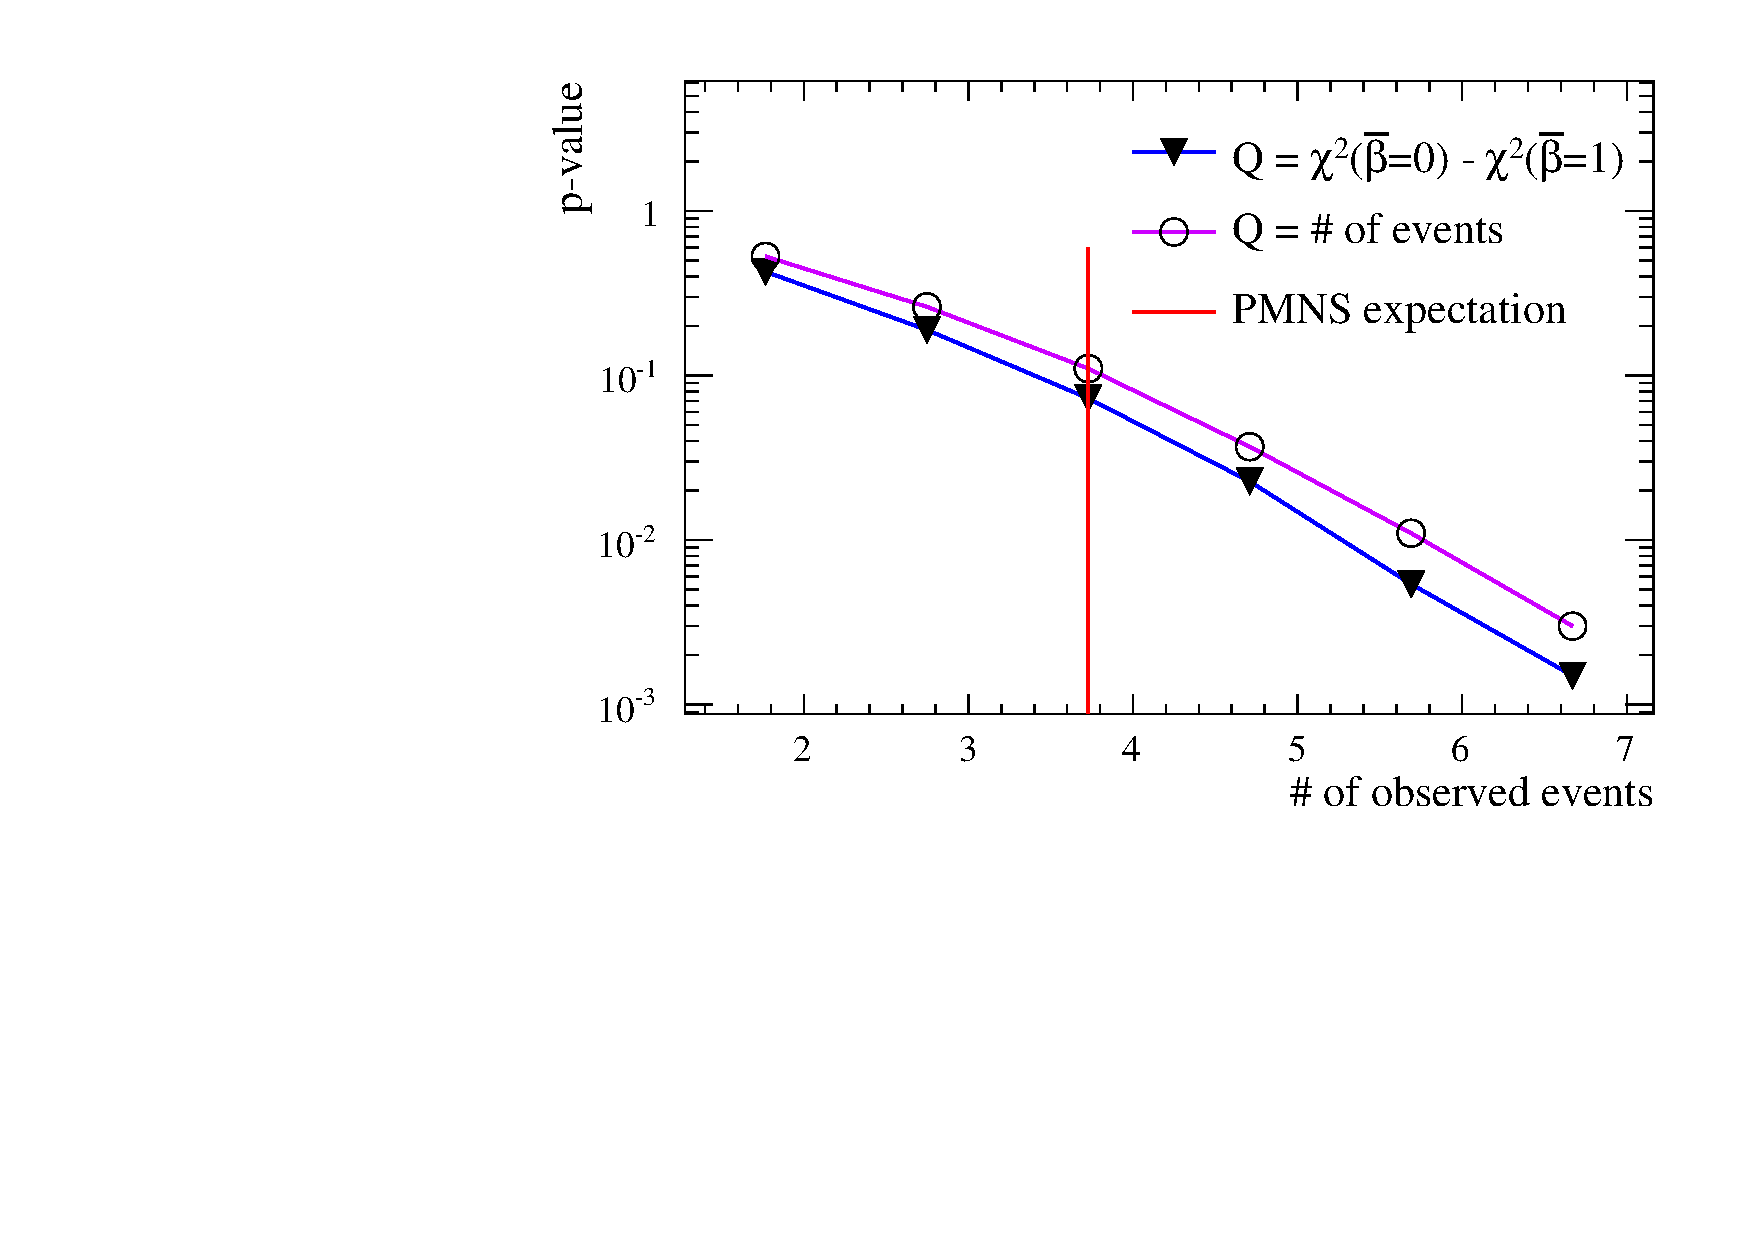
\includegraphics[width=0.48\linewidth]{./nuebar_plots/sensitivity/pvalue_Vs_nevents_4p0108E20POT_log.pdf}
\caption {
Rate-only (violet) and rate+shape (blue) p-value for different number of observed events 
given by Asimov datasets corresponding to the several values of $\beta$ shown in figure~\ref{fig:pvalue_Vs_beta_lowpot}.
Both normal (left) and logarithmic scales (right) are shown.
The red line corresponds to the PMNS expectation ($\beta =1$).
%The study is done with \FakePotLow POT.
The study is done with \TotalPot POT.
\NumToys toys are used.
}
\label{fig:pvalue_Vs_nevents_lowpot}
\end{figure}

%
%\begin{figure}
%\center
%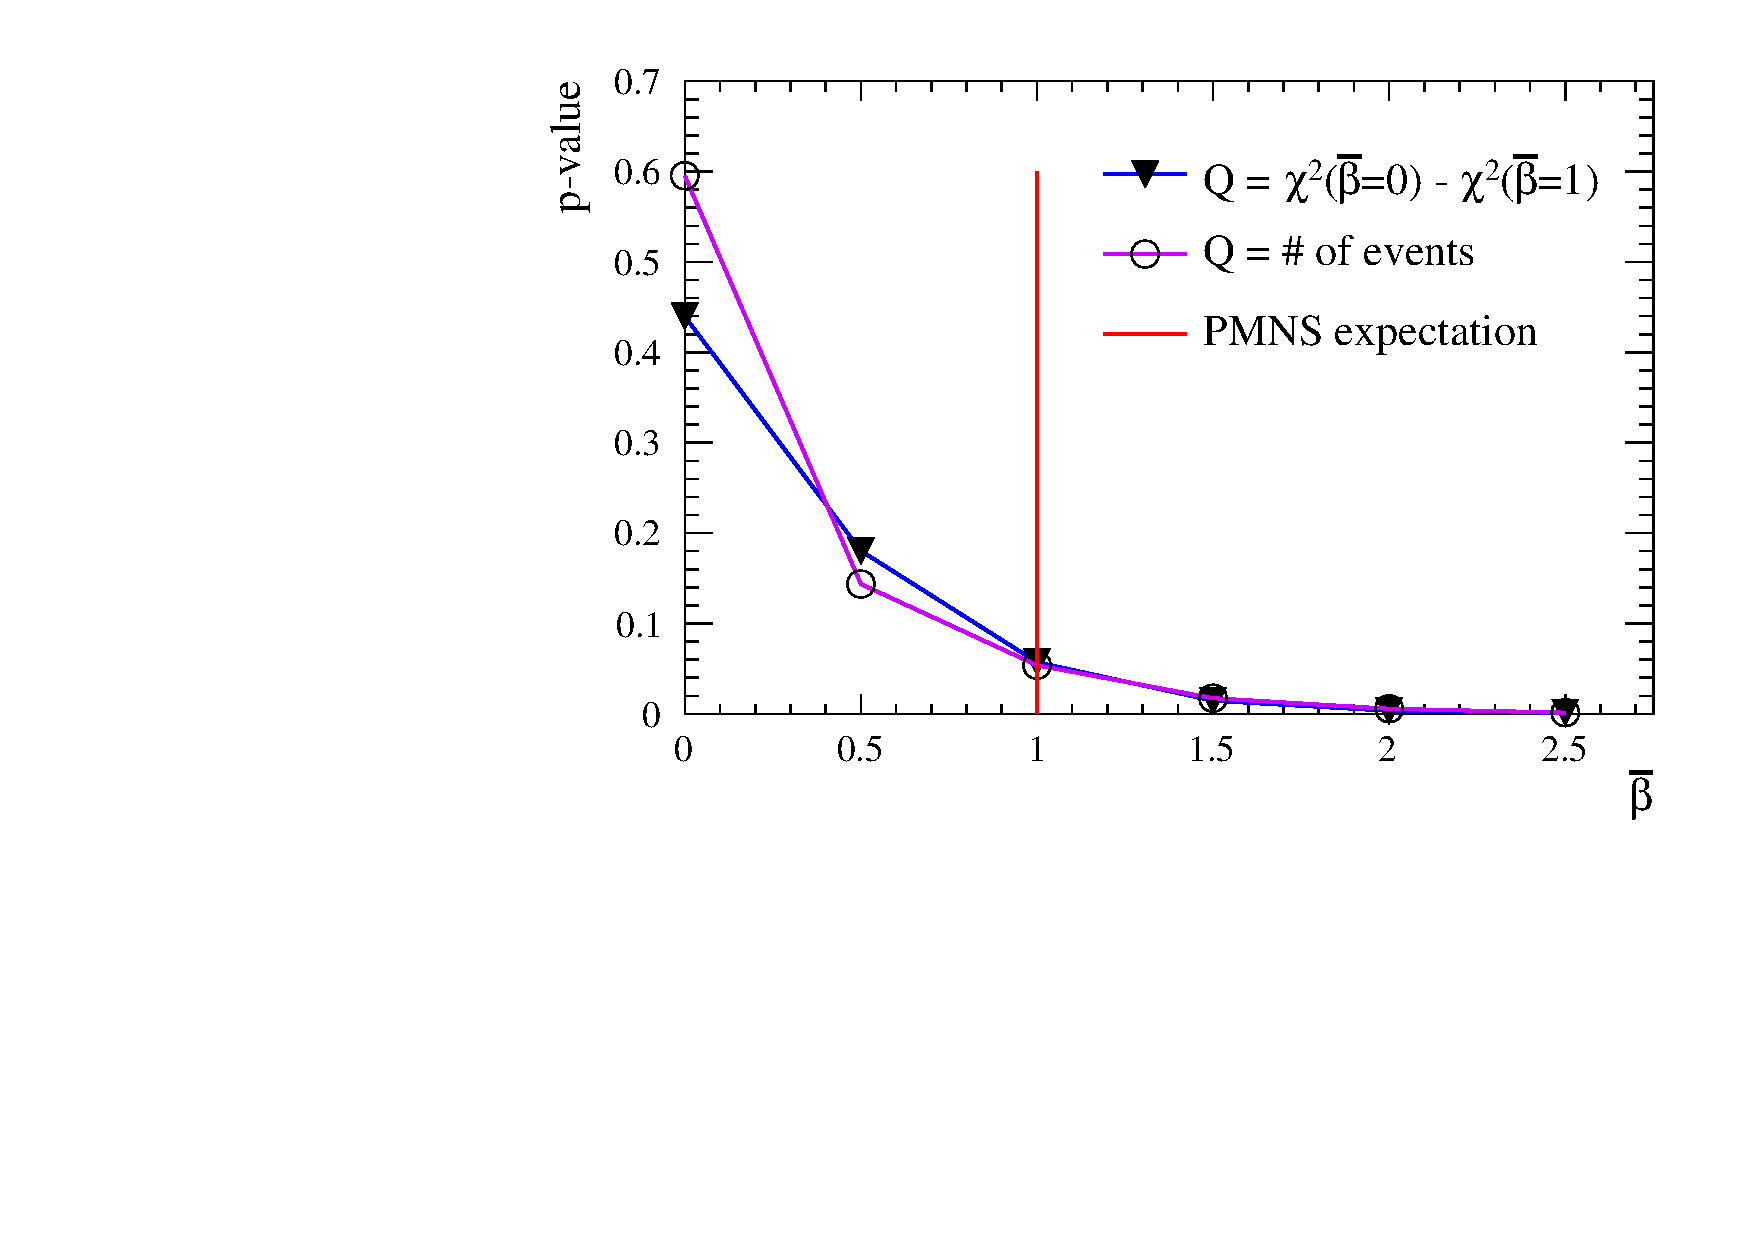
\includegraphics[width=0.48\linewidth]{./nuebar_plots/sensitivity/pvalue_Vs_beta_4p5E20POT.pdf}
%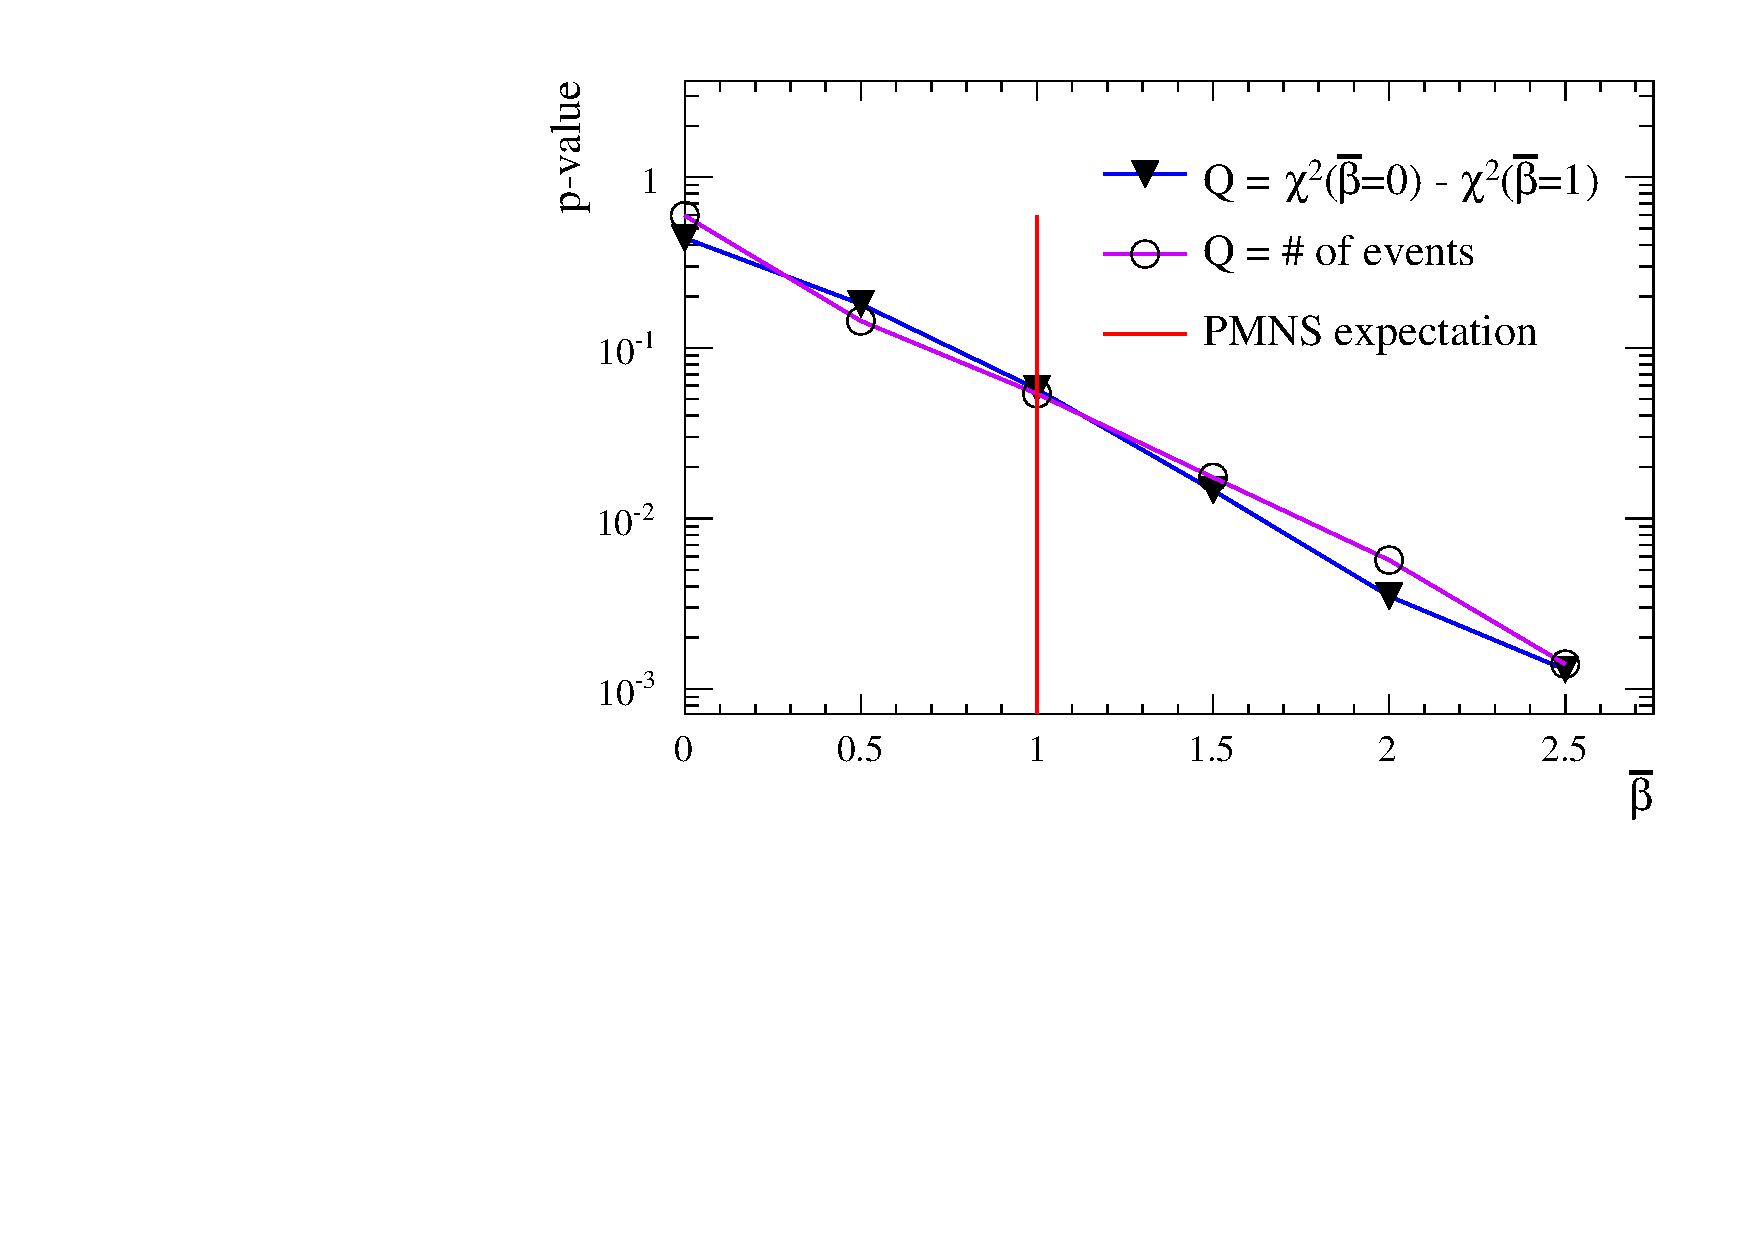
\includegraphics[width=0.48\linewidth]{./nuebar_plots/sensitivity/pvalue_Vs_beta_4p5E20POT_log.pdf}
%\caption {
%Rate-only (violet) and rate+shape (blue) p-value given by Asimov datasets for several values of $\beta$
%in normal (up) and logarithmic (bottom) scale.
%The red line corresponds to the PMNS expectation ($\beta =1$).
%The study is done with 
%\FakePotHigh POT.
%%\newline
%%{\bf TO UPDATE}
%%\newline
%}
%\label{fig:pvalue_Vs_beta_highpot}
%\end{figure}
%
%\begin{figure}
%\center
%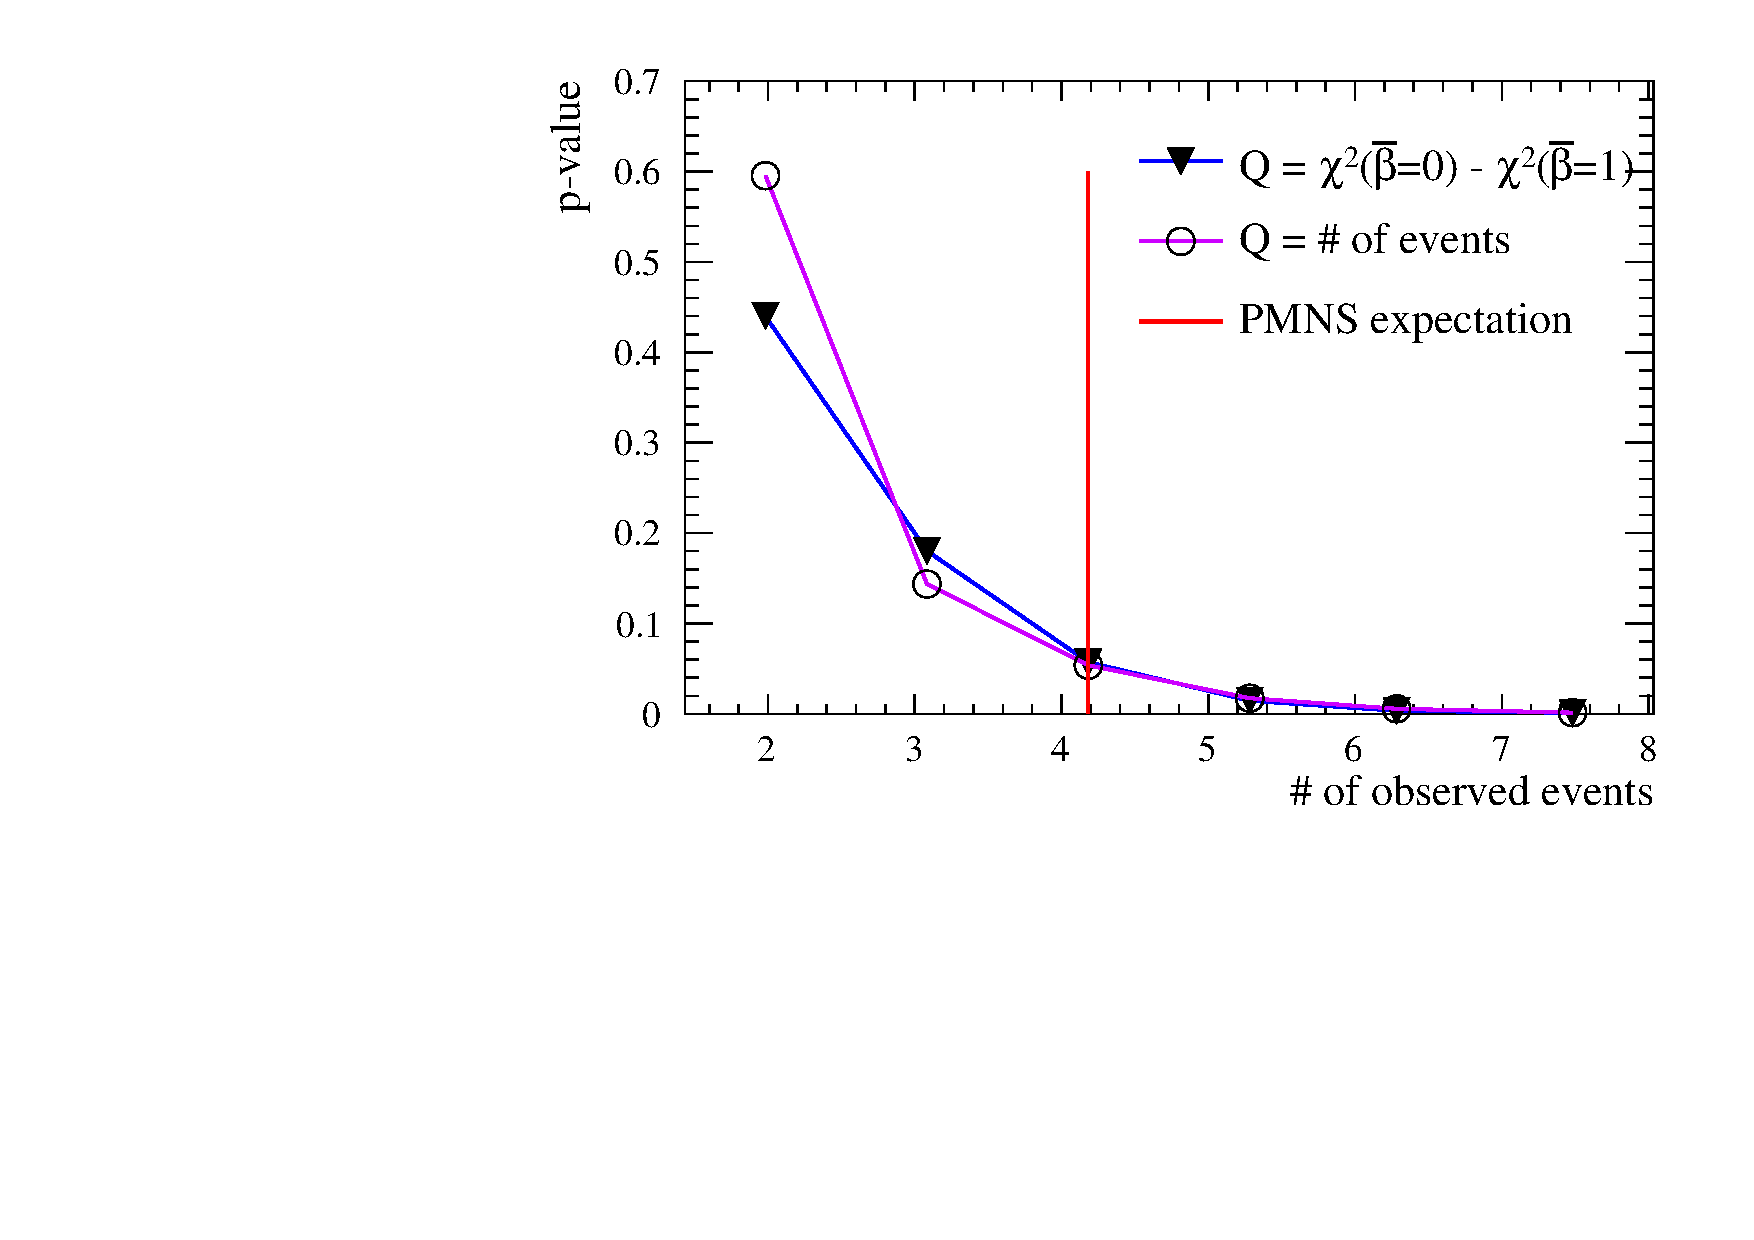
\includegraphics[width=0.48\linewidth]{./nuebar_plots/sensitivity/pvalue_Vs_nevents_4p5E20POT.pdf}
%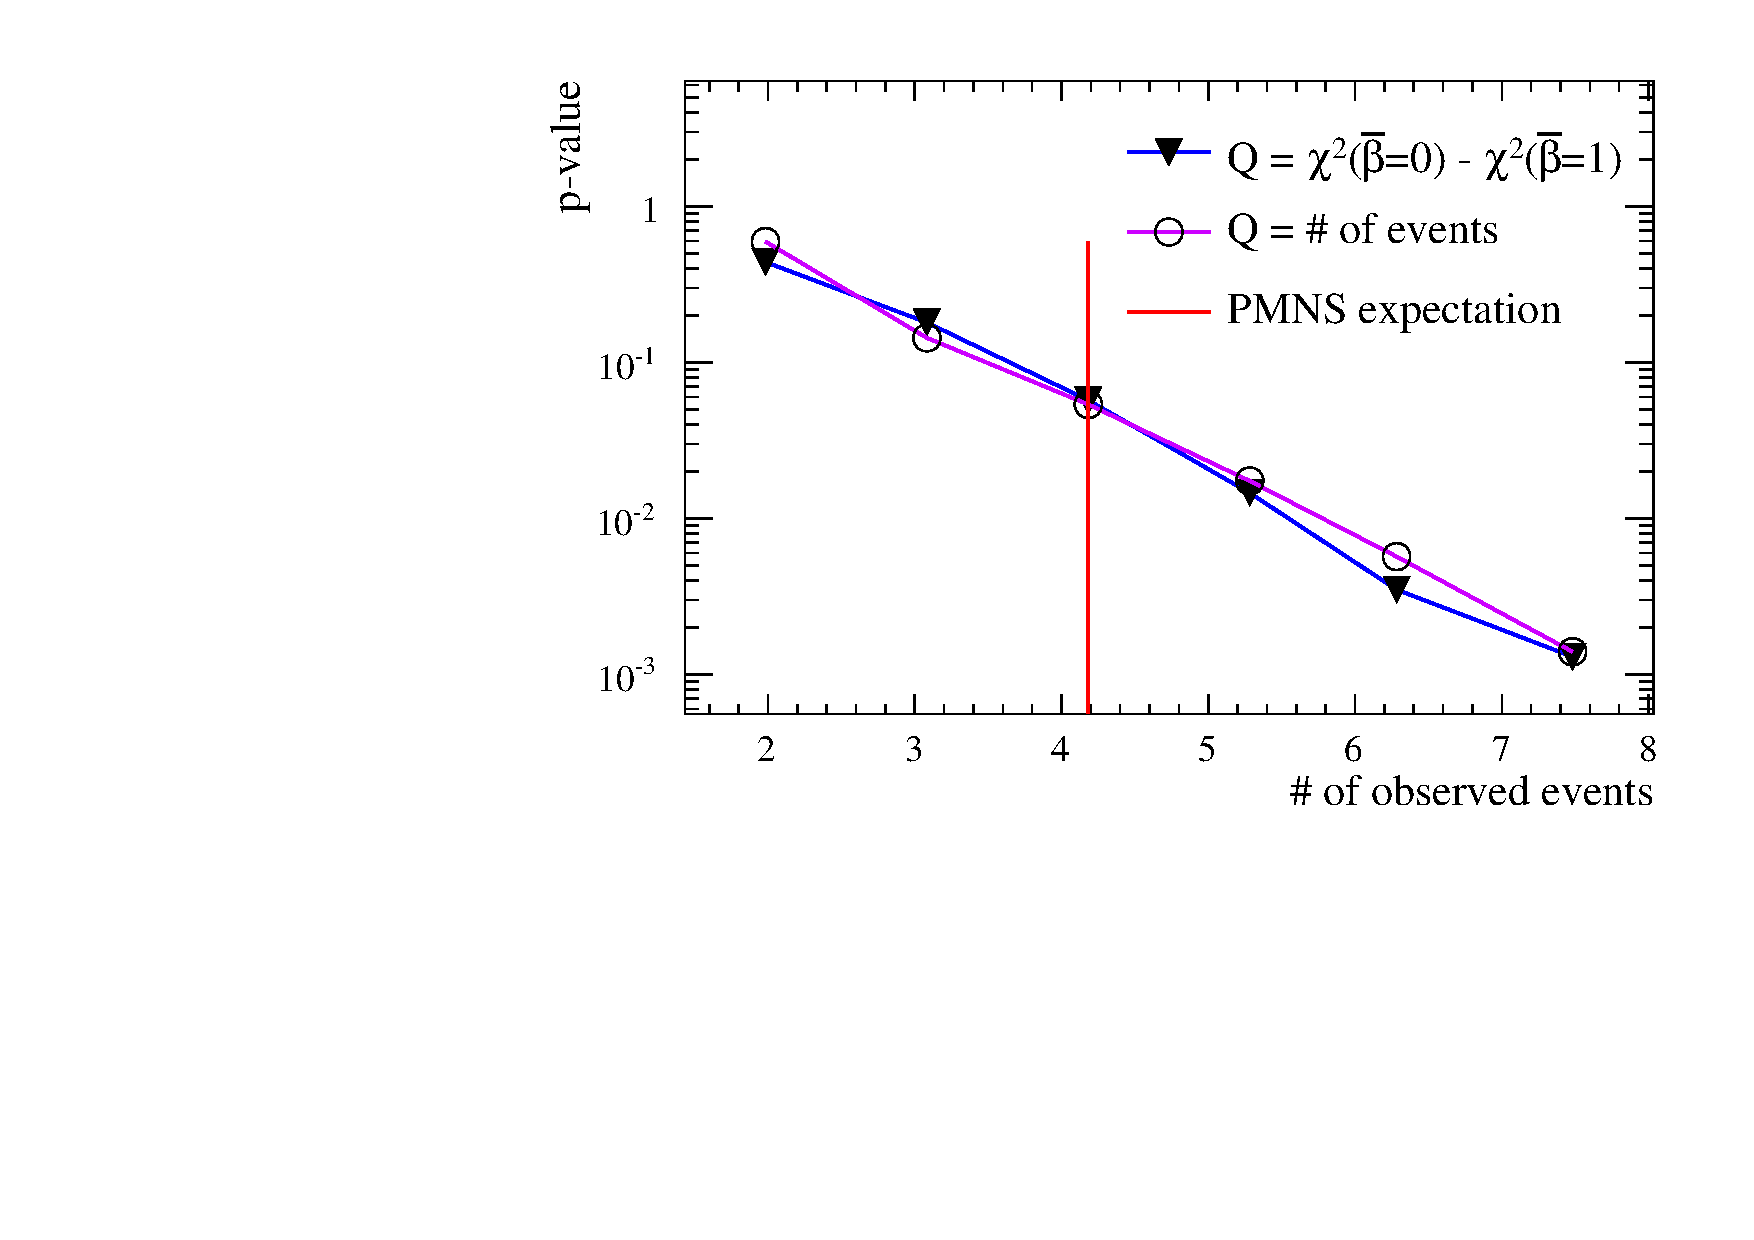
\includegraphics[width=0.48\linewidth]{./nuebar_plots/sensitivity/pvalue_Vs_nevents_4p5E20POT_log.pdf}
%\caption {
%Rate-only (violet) and rate+shape (blue) p-value for different number of observed events 
%given by Asimov datasets corresponding to the several values of $\beta$ shown in ~\ref{fig:pvalue_Vs_beta_highpot}.
%Both normal (up) and logarithmic scales (bottom) are shown.
%The red line corresponds to the PMNS expectation ($\beta =1$).
%The study is done with 
%\FakePotHigh POT.
%%\newline
%%{\bf TO UPDATE}
%%\newline
%}
%\label{fig:pvalue_Vs_nevents_highpot}
%\end{figure}


%--------------------------------------------------------------------------------------------------------------------

\subsection {Mean p-value}
\label{subsec:pvalue_mean}

The mean p-value is computed without using the Asimov dataset, but with toy experiments:
\begin{itemize}
\item the distributions shown in Fig.~\ref{fig:pvalue_rateonly} and Fig.~\ref{fig:pvalue_rateshape} 
	are used respectively for the rate-only and rate+shape p-value computations,
\item \NumToysLarge toys are produced with $\beta = 1$, 
\item for each toy with $\beta=1$ the test statistic (i.e. the number of events and 
	$\Delta \chi^2$ given in Eq.~\ref{eq:deltachisq_rateshape})
	is computed and a 1-sided p-value (right tail) is quoted using the distributions 
	Fig.~\ref{fig:pvalue_rateonly} and Fig.~\ref{fig:pvalue_rateshape}, 
\item a distribution of rate-only and rate+shape p-values is obtained and the mean p-value is calculated.
\end{itemize}

The mean rate-only p-value, given by the mean of the p-value distribution shown in Fig.~\ref{fig:pvalue_mean}, is 0.203
while the mean rate+shape p-value is 0.139  for 
\TotalPot POT.
%\FakePotLow POT.
%For \FakePotHigh POT the rate-only p-value is 0.188 while the rate+shape is 0.127.
%For both cases 
The mean p-value is larger than the Asimov one, which corresponds to the most probable p-value. 
It's worth to point out that this is true on average, but that sometimes it can happen that the rate-only
p-value is smaller than the rate+shape one. This can be due to both the discreteness of the rate-only
p-value or to the shape information wich can discard the $\bar{\nu}_e$ appearance hypothesis.
On average the rate+shape p-value is smaller than the rate-only one,
since it exploits also the shape information, but if a single dataset is used
it can happen that, due to the discreteness of test statistic (number of events), the rate-only p-value
is smaller than the rate+shape p-value.
Indeed a change of the number of events produce a not small jump in the p-value, 
as shown in the left plot of Fig.~\ref{fig:pvalue_mean}, while the distribution of the 
rate+shape p-value is smooth and continuos.
For this reason it is important to quote both the p-values.
 
\begin{figure}
\center
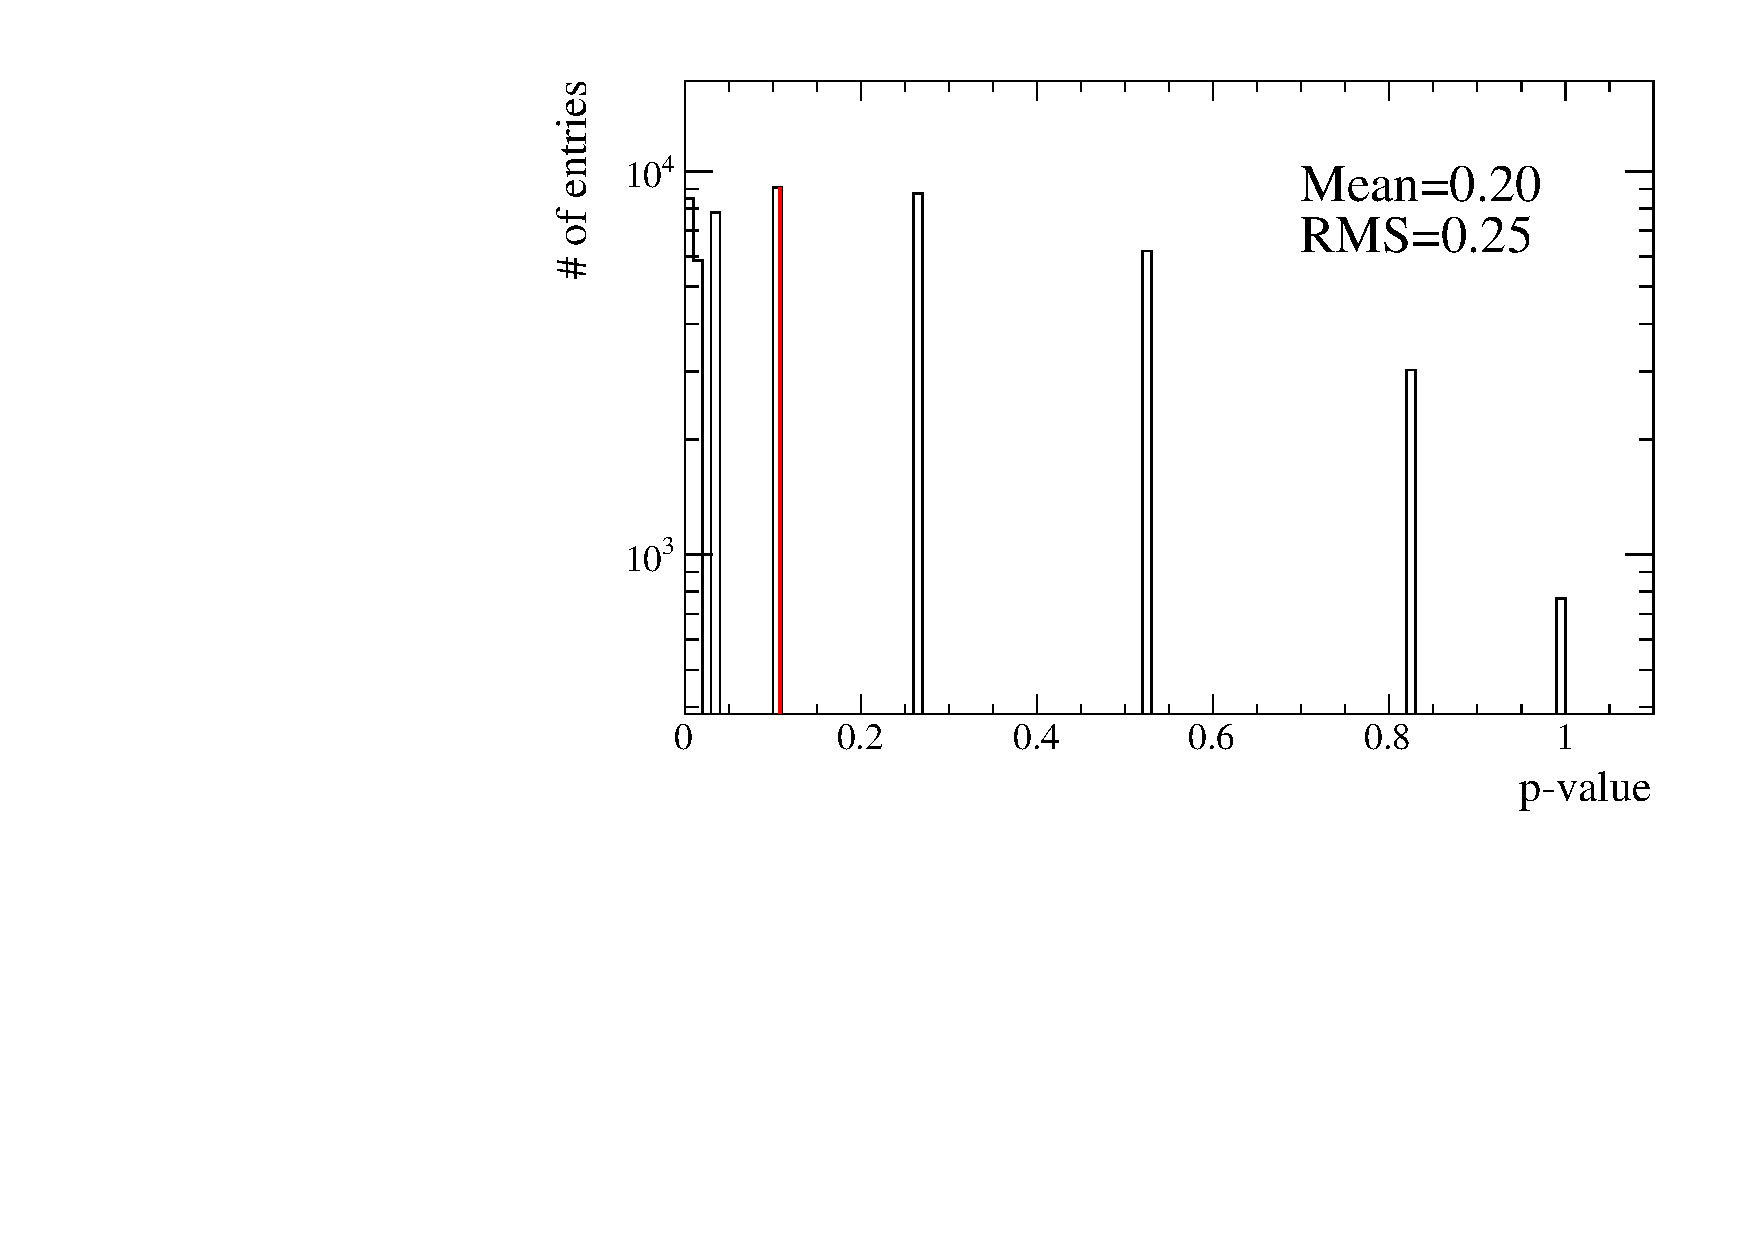
\includegraphics[width=0.48\linewidth]{./nuebar_plots/pvalue_mean/pvalue_rateonly_ave_all_4p0108E20POT_50ktoys.pdf}
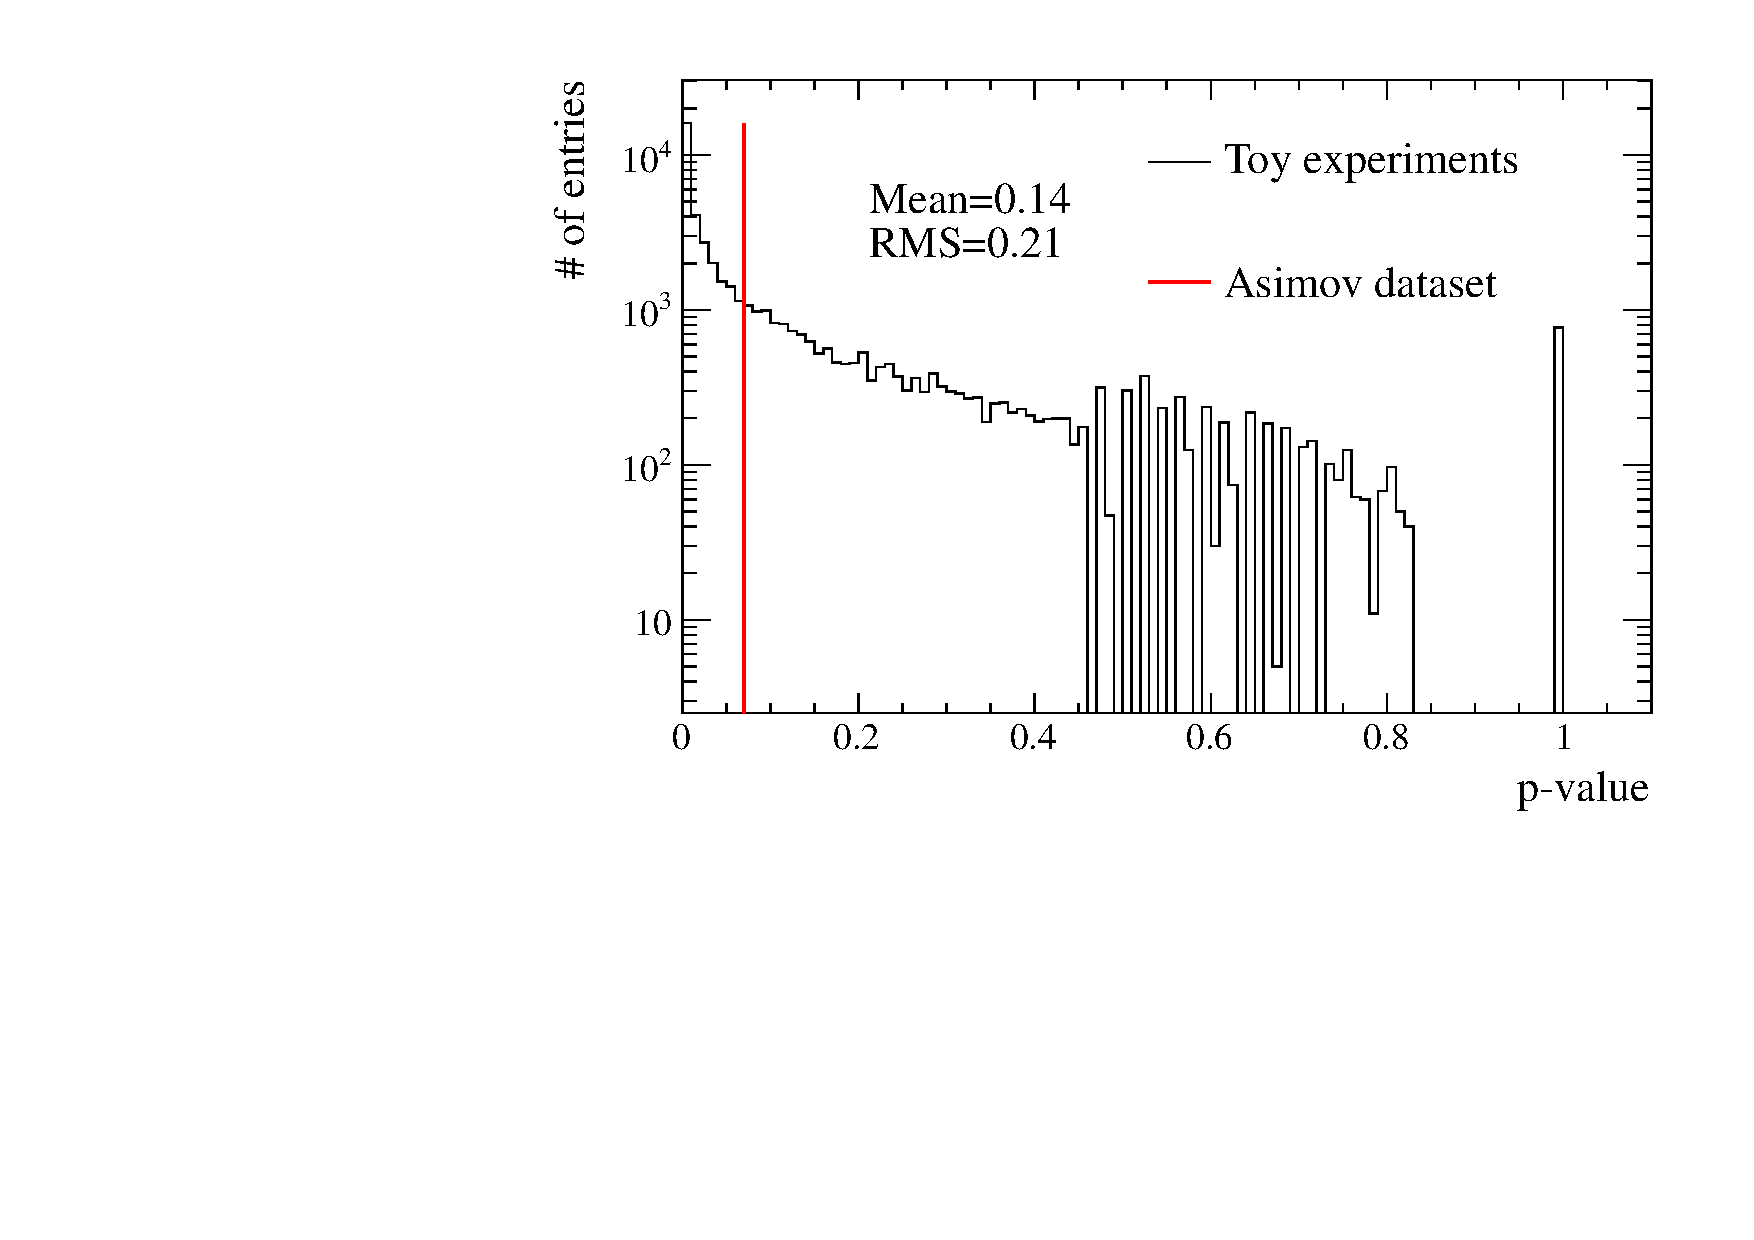
\includegraphics[width=0.48\linewidth]{./nuebar_plots/pvalue_mean/pvalue_rateshape_ave_all_4p0108E20POT_50ktoys.pdf}
%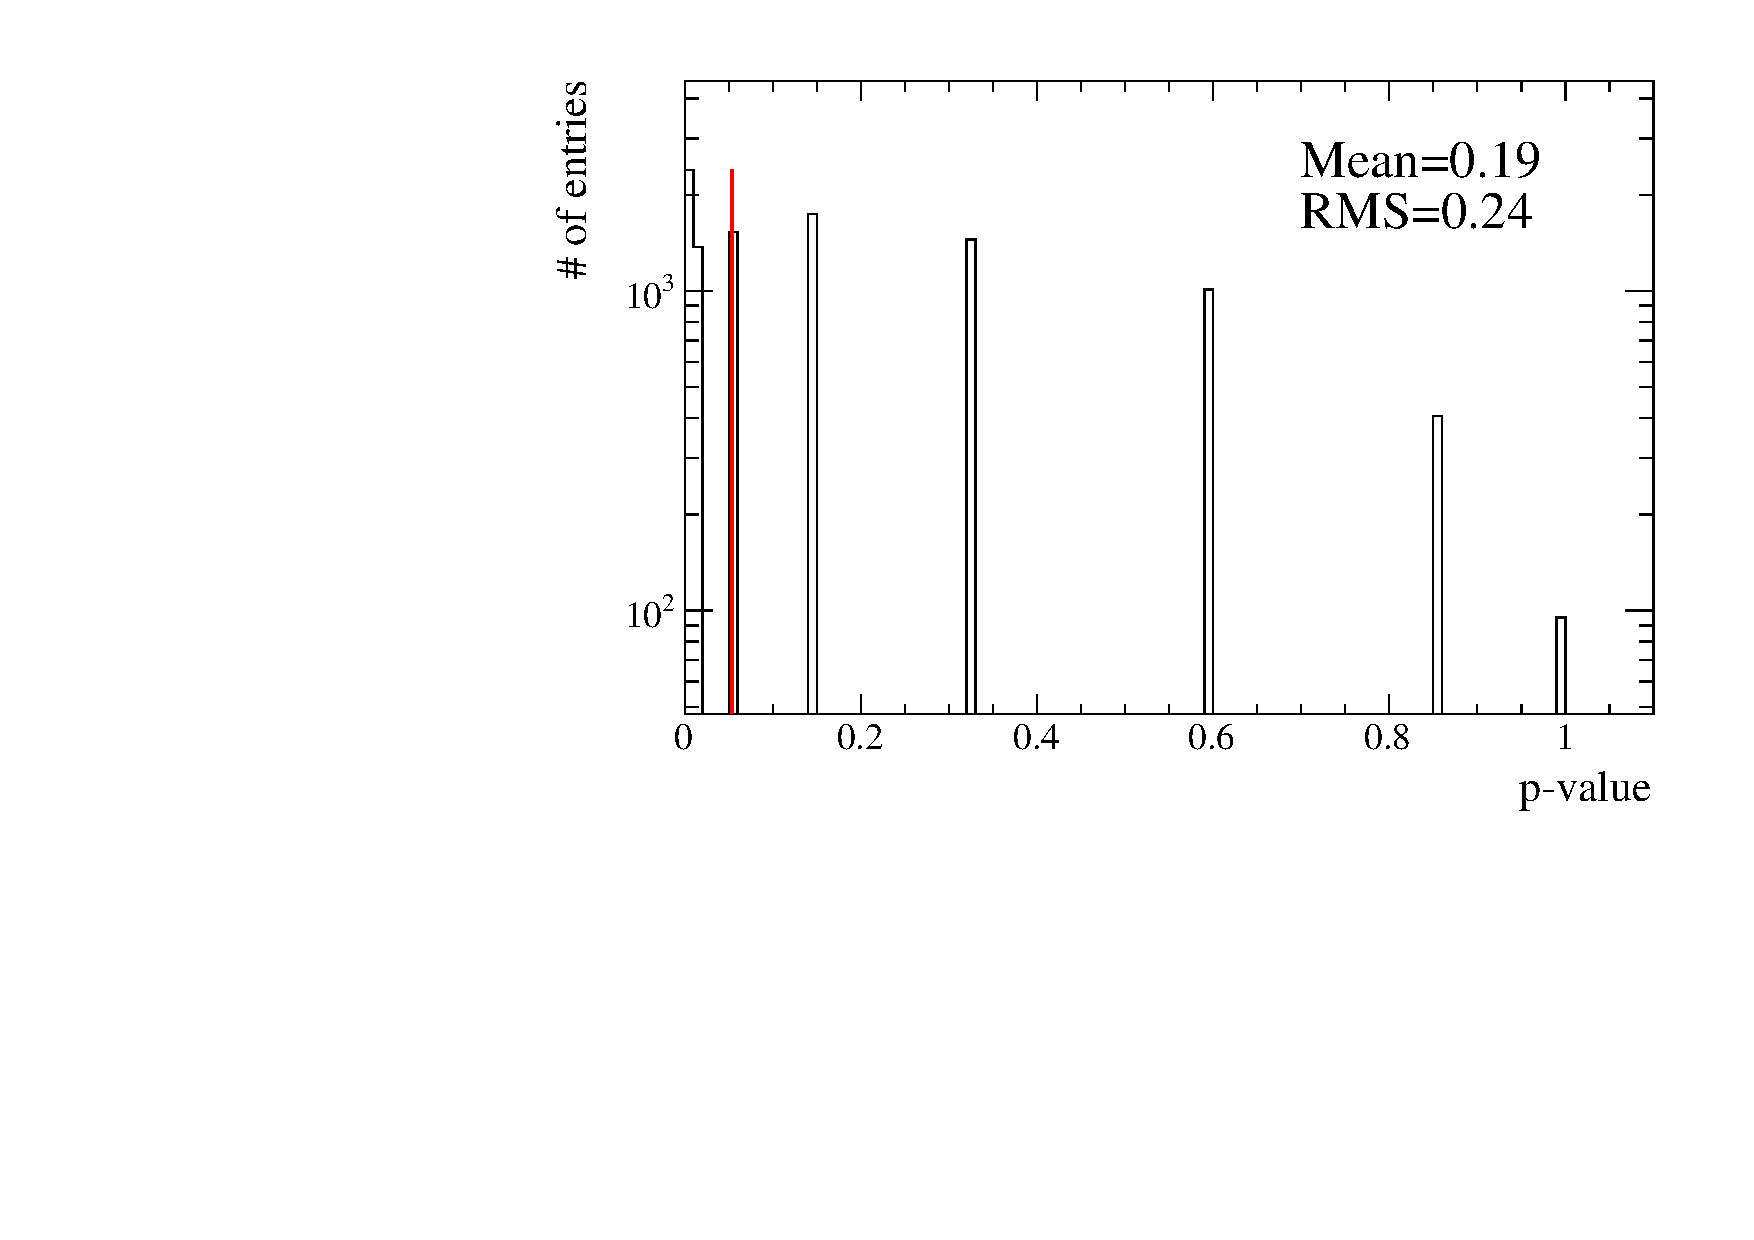
\includegraphics[width=0.48\linewidth]{./nuebar_plots/pvalue_mean/pvalue_rateonly_ave_all_4p5E20POT.pdf}
%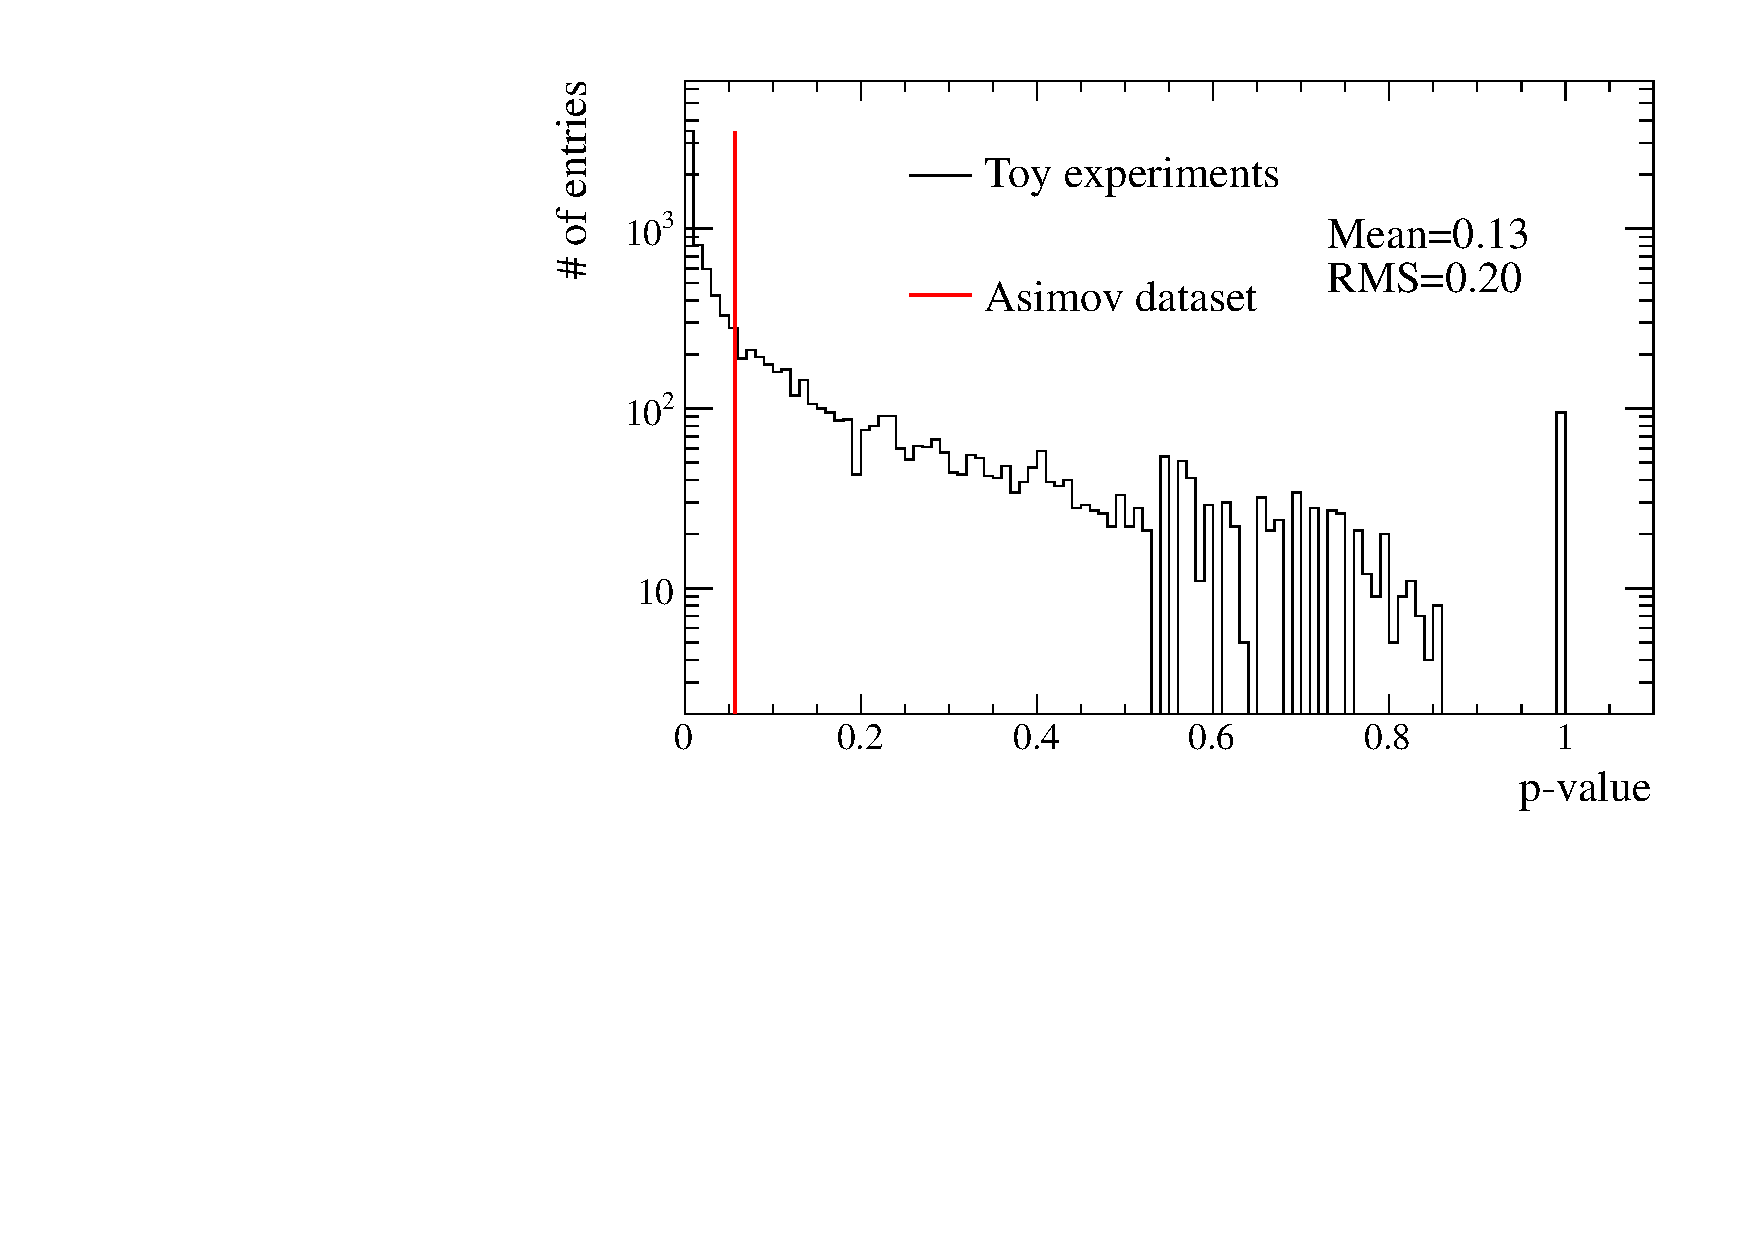
\includegraphics[width=0.48\linewidth]{./nuebar_plots/pvalue_mean/pvalue_rateshape_ave_all_4p5E20POT.pdf}
\caption {
Distribution of rate-only (left) rate+shape (right) p-values obtained by \NumToys toys with $\beta=1$.
The rate-only p-value is discrete and each filled bin correspond to toys with different number of events.
In both distributions the spike at p-value=1 corresponds to toys with no events.
The study is performed with 
\TotalPot POT.
%\FakePotLow (up) \FakePotHigh (down) POT.
\NumToysLarge toys are used.
}
\label{fig:pvalue_mean}
\end{figure}

In Fig.~\ref{fig:pvalue_Vs_nevents_2Dplot} the rate+shape p-value as a function 
of the number of events for single toy produced with $\beta=1$ is shown for \TotalPot POT.

\begin{figure}
\center
%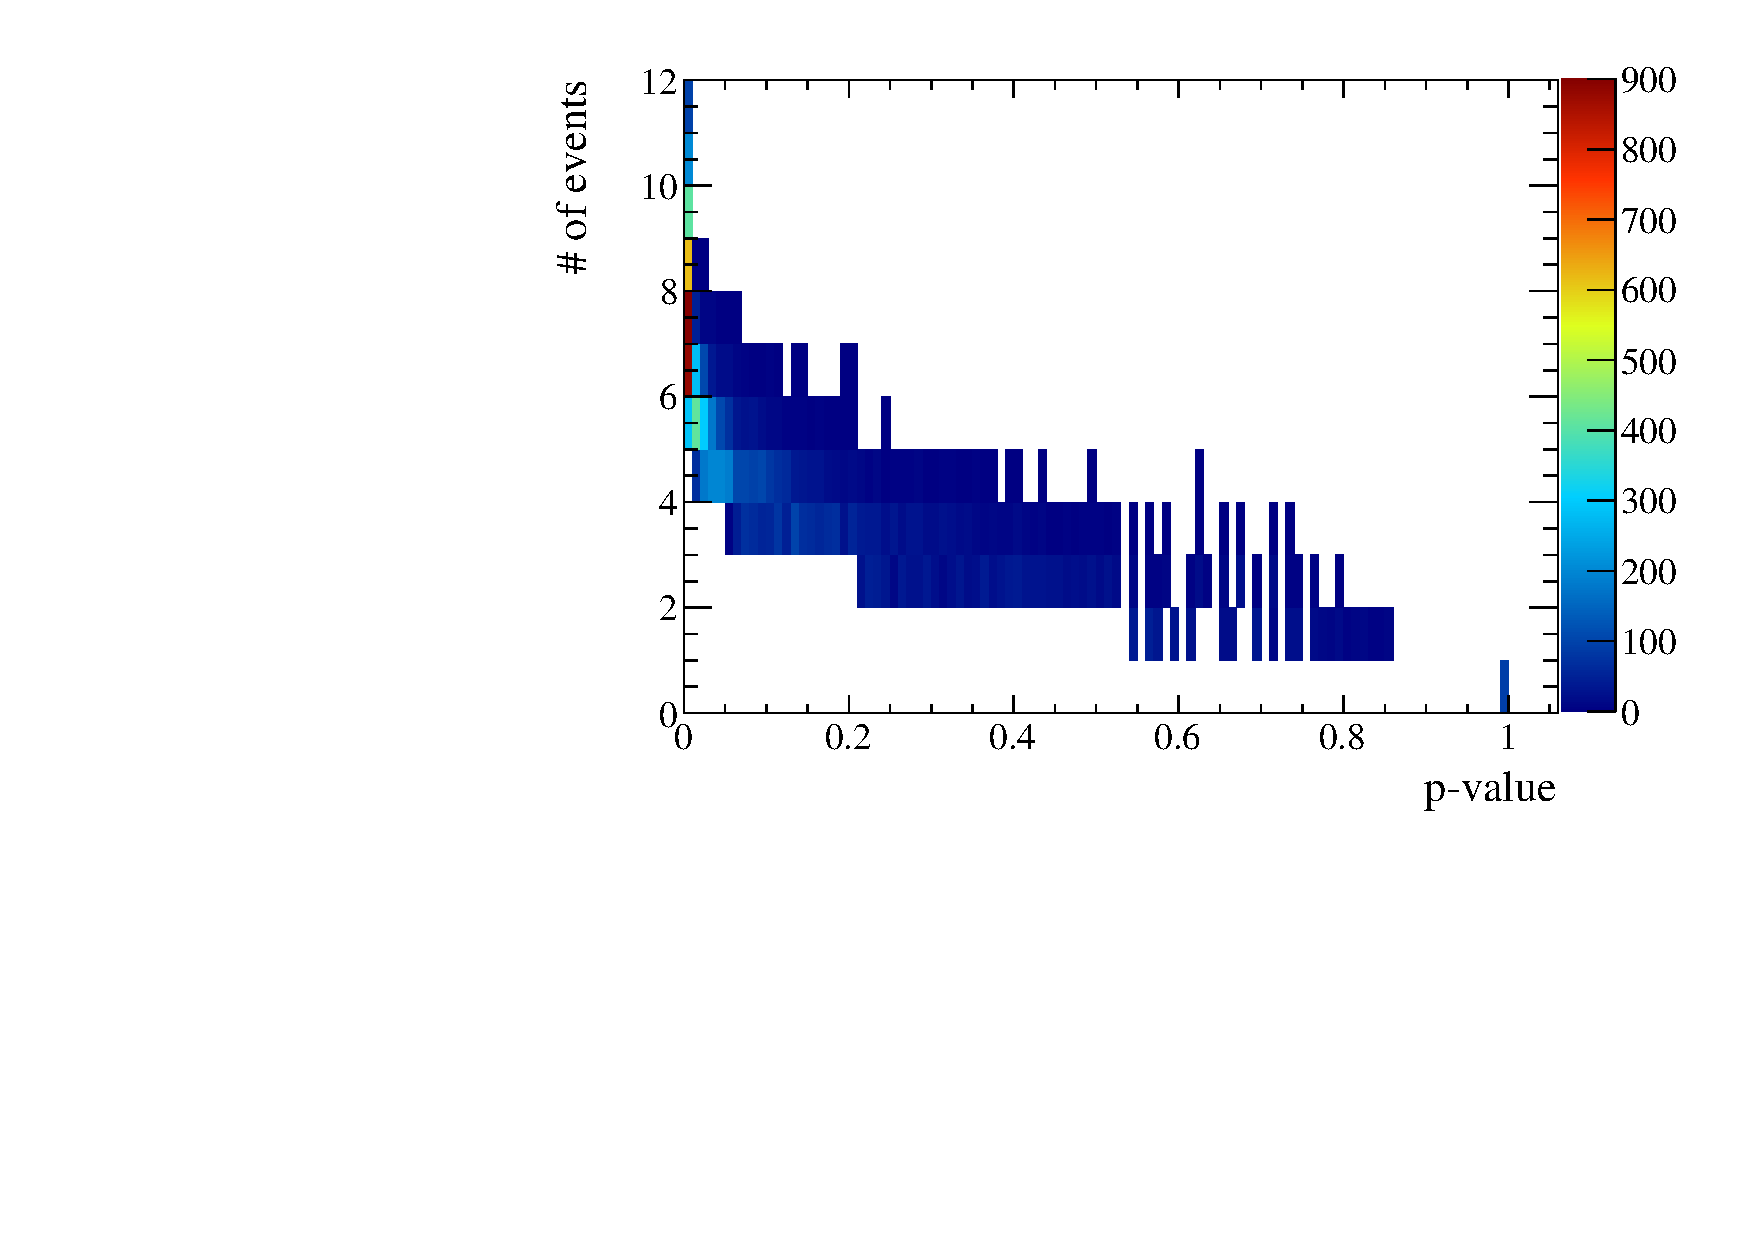
\includegraphics[width=0.48\linewidth]{./nuebar_plots/pvalue_mean/pvalue_Vs_nevents_toy_4p5E20POT}
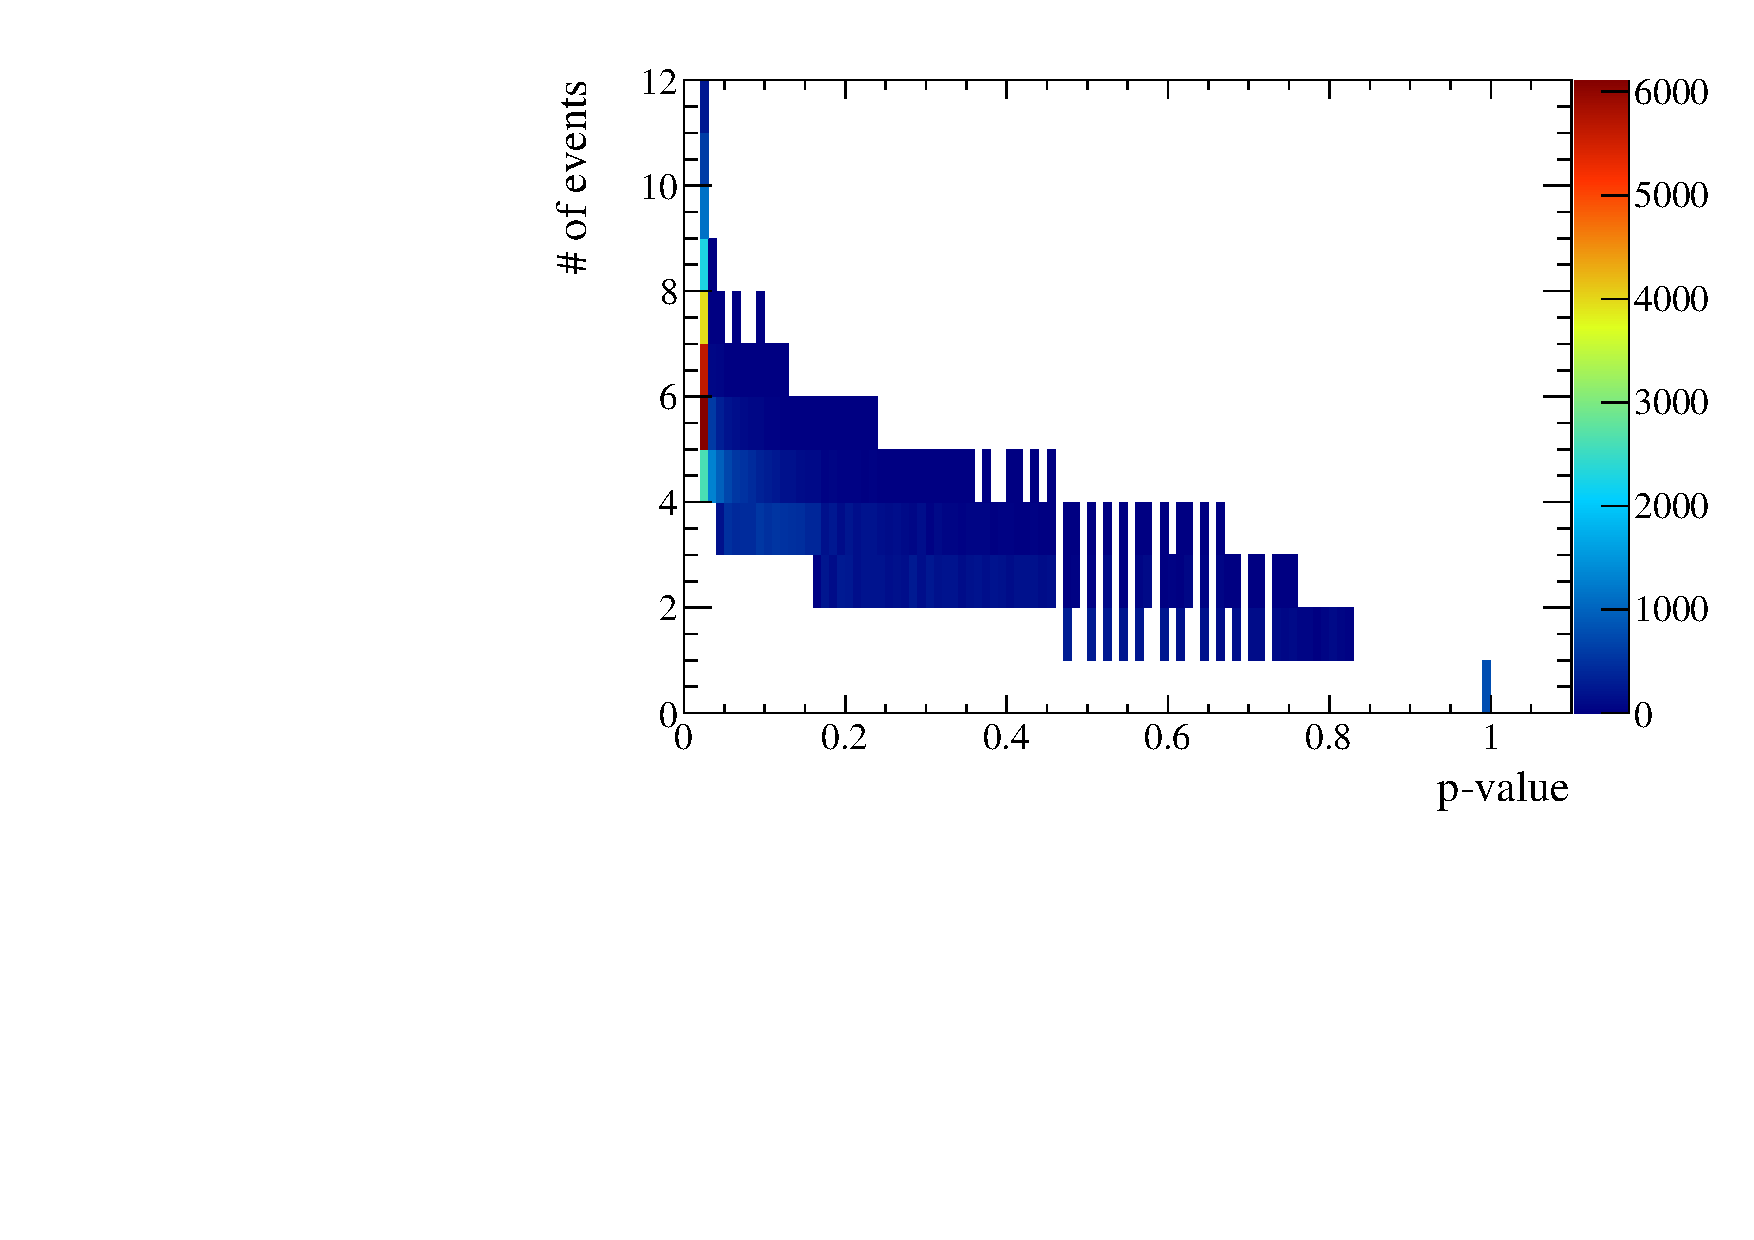
\includegraphics[width=0.6\linewidth]{./nuebar_plots/pvalue_mean/pvalue_Vs_nevents_toy_4p0108E20POT_log_50ktoys}
\caption {
The rate+shape p-value as a function of the number of events for a single toy produced with $\beta=1$ is shown for 
\TotalPot POT.
%\FakePotHigh POT.
\NumToysLarge toys are produced as described in Sec.~\ref{subsec:pvalue_mean}. 
Each entry corresponds to a different toy. 
}
\label{fig:pvalue_Vs_nevents_2Dplot}
\end{figure}



%--------------------------------------------------------------------------------------------------------------------

\subsection {Summary of expected significance to $\bar{\nu}_e$ appearance}
\label{subsec:summary_sensi}

In table~\ref{tab:summary_sensi_lowpot} 
%and table~\ref{tab:summary_sensi_highpot}
the expected rate-only and rate+shape p-values corresponding 
to \TotalPot POT.
%respectively to \FakePotLow POT and \FakePotHigh POT are shown. 
In table
%~\ref{tab:summary_sensi_rateonly_lowpot} and table
~\ref{tab:summary_sensi_rateonly_highpot}
the expected rate-only p-value is shown for different number of observed events
for \TotalPot POT.
%respectively for \FakePotLow POT and \FakePotHigh POT.

In table~\ref{tab:summary_sensi_manytoys} 
it can be seen that the expected p-value is very close to the one computed with \NumToys toys.



\begin{table}
\centering
\begin{tabular}{| c | c |}
\hline
\# of observed events	                                          	& P-value    		    	\\
\hline
$N_{obs} = 2$      		                    	& 0.525                    	\\
$ N_{obs} = 3$      		                    	& 0.264                     	\\
$ \bf N_{obs} = 4$      		                 & \bf 0.109                      	\\
$N_{obs} = 5$      		                    	& 0.0352                      	\\
$N_{obs} = 6$      		                    	& 0.0108                     	\\
\hline
\end{tabular}
\caption{
Summary of the expected rate-only p-values for different number of 
observed events. The simulated number of POT is 
\TotalPot POT.
%\FakePotLow.
\NumToysLarge toys are used to get the distribution of the test statistic and the 
Asimov data is used to compute the p-value.
The Asimov dataset for $\beta=1$ is in bold.
}
\label{tab:summary_sensi_rateonly_highpot}
\end{table}



%\begin{table}
%\centering
%\begin{tabular}{| c | c |}
%\hline
%\# of observed events	                                          	& P-value    		    	\\
%\hline
%$N_{obs} = 2$      		                    	& 0.595                      	\\
%$N_{obs} = 3$      		                    	& 0.322                      	\\
%$N_{obs} = 4$      		                    	& 0.144                    	\\
%$\bf N_{obs} = 5$      		                    	& \bf 0.0538                      	\\
%$N_{obs} = 6$      		                    	& 0.0174                     	\\
%\hline
%\end{tabular}
%\caption{
%Summary of the expected rate-only p-values for different number of 
%observed events. The simulated number of POT is \FakePotHigh.
%\NumToys toys are used to get the distribution of the test statistic and the 
%Asimov data is used to compute the p-value.
%The Asimov dataset for $\beta=1$ is in bold.
%}
%\label{tab:summary_sensi_rateonly_lowpot}
%\end{table}


\begin{table}
\centering
\begin{tabular}{| c | c | c |}
\hline
P-value	                                          	& Asimov    	& Mean 		    	\\
\hline
Rate-only                          			& 0.109           	& 0.203                  	\\
Rate+shape                          		& 0.0699          	& 0.139                  	\\
\hline
\end{tabular}
\caption{
Summary of the expected rate-only and rate+shape p-values for 
\TotalPot POT.
%\FakePotLow POT.
The Asimov p-value is calculated using the Asimov dataset while the 
mean p-value is calculated making \NumToysLarge toys and taking the mean 
of the p-value distribution.
}
\label{tab:summary_sensi_lowpot}
\end{table}

%\begin{table}
%\centering
%\begin{tabular}{| c | c | c |}
%\hline
%P-value	                                          	& Asimov    	& Mean 		    	\\
%\hline
%Rate-only                          			& 0.0538           & 0.188                   	\\
%Rate+shape                          		& 0.0572          	& 0.127                  	\\
%\hline
%\end{tabular}
%\caption{
%Summary of the expected rate-only and rate+shape p-values for \FakePotHigh POT.
%The Asimov p-value is calculated using the Asimov dataset while the 
%mean p-value is calculated making \NumToys toys and taking the mean 
%of the p-value distribution.
%}
%\label{tab:summary_sensi_highpot}
%\end{table}
%






% Comparison with many toys

\begin{table}
\centering
\begin{tabular}{| c | c | c |}
\hline
P-value	                                          	& Asimov    	& Mean 		    	\\
\hline
Rate-only (\NumToys toys)         			& 0.110           	& 0.207                  	\\
Rate+shape (\NumToys toys)              		& 0.0726          	& 0.143                  	\\
\hline
Rate-only (\NumToysLarge toys)        			& 0.109           & 0.203                	\\
Rate+shape (\NumToysLarge toys)             		& 0.0699          	& 0.139                	\\
\hline
\end{tabular}
\caption{
Summary of the expected rate-only and rate+shape p-values for 
\TotalPot POT, using \NumToys (up) and \NumToysLarge (bottom) toys for fake datasets (both $\beta=0$ and $\beta=1$).
The Asimov p-value is calculated using the Asimov dataset while the mean one
from \NumToys (up) and \NumToysLarge (bottom) toys and taking the mean 
of the p-value distribution.
}
\label{tab:summary_sensi_manytoys}
\end{table}


\begin{table}
\centering
\begin{tabular}{| c | c | c |}
\hline
P-value	                                          	& Asimov    	& Mean 		    	\\
\hline
Rate-only (\NumToys toys)        			& 0.0343           & 0.1004                   	\\
Rate+shape (\NumToys toys)             		& 0.0249          	& 0.0649                 	\\
\hline
Rate-only (\NumToysLarge toys)        			& 0.0331           & 0.1007                   	\\
Rate+shape (\NumToysLarge toys)             		& 0.0243          	& 0.0660                 	\\
\hline
\end{tabular}
\caption{
Summary of the expected rate-only and rate+shape p-values for 
$8 \times 10^{20}$ POT, using \NumToys (up) and \NumToysLarge (bottom) toys for fake datasets (both $\beta=0$ and $\beta=1$).
The Asimov p-value is calculated using the Asimov dataset while the mean one
from \NumToys (up) and \NumToysLarge (bottom) toys and taking the mean 
of the p-value distribution.
}
\label{tab:summary_sensi_manytoys}
\end{table}

%





\begin{table}
\centering
\begin{tabular}{| c | c | c |}
\hline
		                                          	& p-value $\leq 0.10$    		& p-value $\leq 0.05$ 		\\
\hline
Fraction of toys	(rate-only)			& 44.3\%					& 44.3\%				\\
Fraction of toys	(rate+shape) 		& 64.0\%					& 52.8\%				\\
\hline
\end{tabular}
\caption{
The probability to have a p-value smaller than 0.05 and 0.10 is shown.
\NumToysLarge toys for
%\FakePotLow POT 
\TotalPot POT
are produced.
Then for each toy the p-value is computed as described in section~\ref{subsec:pvalue_mean}.
}
\label{tab:pvalue_mean_0p05_lowpot}
\end{table}

%
%\begin{table}
%\centering
%\begin{tabular}{| c | c | c |}
%\hline
%		                                          	& p-value $\leq 0.10$    		& p-value $\leq 0.05$     	\\
%\hline
%%Mean p-value (rate-only) 			&  0.0213     				&  0.00809                  	\\
%Fraction of toys	(rate-only)			& 53.0\%					&  37.7\%				\\
%%Mean p-value (rate+shape)       		&  0.0214    				&  0.0118                  	\\
%Fraction of toys	(rate+shape) 		& 67.1\%					&  56.6\%				\\
%\hline
%\end{tabular}
%\caption{
%The probability to have a p-value smaller than 0.05 and 0.10 is shown.
%\NumToys toys for \FakePotHigh POT are produced.
%Then for each toy the p-value is computed as described in~\ref{subsec:pvalue_mean}.
%}
%\label{tab:pvalue_mean_0p05_highpot}
%\end{table}
%
%


\begin{table}
\centering
\begin{tabular}{| c | c | c |}
\hline
\# obs events $>$ \# exp bkg		& p-value    	 & Fraction of toys    	\\
\hline
Rate-only                          			&   0.149    	& 92.4\%             	\\
Rate+shape                          		&   0.0927   	& 92.4\%                 	\\
\hline
\end{tabular}
\caption{
Summary of the expected rate-only and rate+shape mean p-values for 
\TotalPot POT.
%\FakePotLow POT.
The Asimov p-value is calculated using the Asimov dataset while the 
mean p-value is calculated making \NumToysLarge toys and taking the mean 
of the p-value distribution.
Only fake datasets with number of observed events higher than the
expected background are considered.
The fraction of selected toys is shown as well. 
}
\label{tab:pvalue_mean_bkg_lowpot}
\end{table}

%
%\begin{table}
%\centering
%\begin{tabular}{| c | c | c |}
%\hline
% \# obs events $>$ \# exp bkg           & P-value  	 & Fraction of toys    	\\
%\hline
%Rate-only                          			&  0.151      	&   95\%               	\\
%Rate+shape                          		&  0.0947    	&   95\%             	\\
%\hline
%\end{tabular}
%\caption{
%Summary of the expected rate-only and rate+shape mean p-values for \FakePotHigh POT.
%The Asimov p-value is calculated using the Asimov dataset while the 
%mean p-value is calculated making \NumToys toys and taking the mean 
%of the p-value distribution.
%Only fake datasets with number of observed events higher than the
%expected background are considered.
%The fraction of selected toys is shown as well. 
%}
%\label{tab:pvalue_mean_bkg_highpot}
%\end{table}


\begin{table}
\centering
\begin{tabular}{| c | c |}
\hline
p-value (rate-only) $>$ p-value (rate+shape)		& Probability          	\\
\hline
All toys									& 85.0\%									\\
Toys w/ \# obs. events $>$ \# exp. bkg 			& 77.4\%									\\
\hline
\end{tabular}
\caption{
The probability to have a rate-only p-value larger than the rate+shape p-value is shown.
\NumToysLarge toys for 
\TotalPot POT.
%\FakePotLow POT are produced.
Then for each toy the p-value is computed as described in section~\ref{subsec:pvalue_mean}.
Both all toys are considered as well as the toys with the number of observed events larger
than the number of expected background.
}
\label{tab:pvalue_mean_rate_large_shape_lowpot}
\end{table}


%\begin{table}
%\centering
%\begin{tabular}{| c | c |}
%\hline
%p-value (rate-only) $>$ p-value (rate+shape)		& Probability          	\\
%\hline
%All toys									& 81.4\%									\\
%Toys w/ \# obs. events $>$ \# exp. bkg 			& 77.4\%									\\
%\hline
%\end{tabular}
%\caption{
%The probability to have a rate-only p-value larger than the rate+shape p-value is shown.
%\NumToys toys for \FakePotHigh POT are produced.
%Then for each toy the p-value is computed as described in~\ref{subsec:pvalue_mean}.
%Both all toys are considered as well as the toys with the number of observed events larger
%than the number of expected background.
%}
%\label{tab:pvalue_mean_rate_large_shape_highpot}
%\end{table}



The mean rate-only and rate+shape p-values, obtained considering only p-values smaller than 0.05 (0.10), 
are shown table~\ref{tab:pvalue_mean_0p05_lowpot}.
% and in table~\ref{tab:pvalue_mean_0p05_highpot}.
The corresponding figures are shown in appendix~\ref{app:rateshape_mean_pvalue}.

In table~\ref{tab:pvalue_mean_bkg_lowpot}
% and table~\ref{tab:pvalue_mean_bkg_highpot} the 
mean p-values corresponding to 
\TotalPot POT
%\FakePotLow POT and \FakePotHigh POT are shown
for those fake datasets with the number of observed events higher than the expected background are shown. 

In table~\ref{tab:pvalue_mean_rate_large_shape_lowpot} 
%and table~\ref{tab:pvalue_mean_rate_large_shape_highpot}
the probability to have the rate-only p-value smaller than the rate+shape p-value is shown for
\TotalPot POT.
%\FakePotLow POT and \FakePotHigh POT.

















